\documentclass[11pt]{article}

\usepackage[a4paper,margin=1in]{geometry}
\usepackage{amsmath,amssymb}
\usepackage{booktabs}
\usepackage{caption}
\usepackage{enumitem}
\usepackage{graphicx}
\usepackage{listings}
\usepackage{mdframed}
\usepackage{microtype}
\usepackage{placeins}
\usepackage{tabularx}
\usepackage{xcolor}
\usepackage{tikz}
\usetikzlibrary{arrows.meta,calc,decorations.pathreplacing,fit,positioning}
\usepackage{hyperref}

\definecolor{nvidiagreen}{HTML}{76B900}
\captionsetup{labelsep=period}
\definecolor{codebg}{HTML}{F6F8FA}
\definecolor{codecomment}{HTML}{527A3A}
\definecolor{codekeyword}{HTML}{7A3E9D}
\definecolor{codestring}{HTML}{A03B32}

\hypersetup{
  colorlinks=true,
  linkcolor=blue!55!black,
  citecolor=blue!55!black,
  urlcolor=blue!55!black,
}

\setlength{\parindent}{0pt}
\setlength{\parskip}{0.55em}
\setcounter{tocdepth}{2}
\numberwithin{equation}{section}
\numberwithin{figure}{section}
\numberwithin{table}{section}
\setlist[itemize]{leftmargin=*,itemsep=0.25em,topsep=0.35em}
\setlist[enumerate]{leftmargin=*,itemsep=0.25em,topsep=0.35em}
\renewcommand{\arraystretch}{1.15}
\newcolumntype{Y}{>{\raggedright\arraybackslash}X}

\lstdefinelanguage{CUDA}{
  language=C++,
  morekeywords={
    __global__,__device__,__host__,
    cudaError_t,cudaSuccess,cudaMallocManaged,cudaFree,
    cudaDeviceSynchronize,cudaGetDevice,cudaMemPrefetchAsync,
    cudaGetErrorString,cudaGetLastError,
    threadIdx,blockIdx,blockDim,gridDim,cudaCpuDeviceId
  },
  sensitive=true,
}

\lstset{
  basicstyle=\ttfamily\small,
  backgroundcolor=\color{codebg},
  commentstyle=\color{codecomment},
  keywordstyle=\color{codekeyword}\bfseries,
  stringstyle=\color{codestring},
  numbers=left,
  numberstyle=\scriptsize\color{black!55},
  numbersep=8pt,
  frame=single,
  rulecolor=\color{black!20},
  breaklines=true,
  columns=fullflexible,
  keepspaces=true,
  showstringspaces=false,
  tabsize=2,
  aboveskip=0.8em,
  belowskip=0.8em,
}

\newcommand{\code}[1]{\texttt{#1}}
\newcommand{\CUDA}{\textsc{Cuda}}
\newcommand{\CPU}{\textsc{Cpu}}
\newcommand{\GPU}{\textsc{Gpu}}
\newcommand{\bigO}{\mathcal{O}}

\newenvironment{physicsview}{%
  \begin{mdframed}[
    backgroundcolor=nvidiagreen!6,
    linecolor=nvidiagreen!65!black,
    linewidth=0.7pt,
    nobreak=true,
    innerleftmargin=8pt,
    innerrightmargin=8pt,
    innertopmargin=7pt,
    innerbottommargin=7pt
  ]
  \textbf{Physics viewpoint.}\par
}{%
  \end{mdframed}
}

\title{GPU Computing and CUDA}
\author{}
\date{Reference prepared September 2026}

\begin{document}

\hypersetup{pageanchor=false}
\maketitle

\begin{abstract}
This reference builds a CUDA mental model around one array-addition example.
Section 1 defines the CPU, GPU, host memory, device memory, and CUDA execution
model, then places those definitions in an A100 and an RTX 3090.  Section 2
develops and measures the addition kernel.  Section 3 uses
eight pairs of small programs to show why a GPU may wait or do unnecessary work.
\end{abstract}

\clearpage
\hypersetup{pageanchor=true}
\pagenumbering{roman}
\tableofcontents
\clearpage
\pagenumbering{arabic}

\section{GPU and CUDA}

% ============================================================================
\subsection{CPU and GPU interaction}
\label{chap:origins}
\label{chap:getting-started}
% ============================================================================

A discrete GPU normally works alongside the CPU in the same computer.  This is true
for a data-center GPU or a workstation GPU.
CUDA calls the computer that runs the CPU code the host.  The host's main RAM
(random-access memory) is called host memory and normally uses DDR (double data
rate) DRAM (dynamic random-access memory).  A discrete GPU has separate device memory,
which is also DRAM.  Data-center GPUs usually use HBM (high-bandwidth memory), while
consumer GPUs usually use GDDR (graphics double data rate) memory
\cite{ampere2020,ga102whitepaper}.  This section assumes a discrete GPU.  An
integrated GPU may instead share system DRAM with the CPU.

The CPU runs the main program and launches a GPU kernel for work that can be split
among many threads~\cite{gupta2020origins}.  Figure~\ref{fig:cpu-gpu-interaction}
shows the complete interaction.

For informal discussion, this note calls kernel work either \emph{computation} or
\emph{logistics}.  These are not CUDA terms.
\begin{itemize}
  \item A \emph{computation kernel} performs the numerical operation of interest.
  \item A \emph{logistics kernel} prepares data for another kernel, for example by
  transposing, gathering, scattering, packing, or unpacking the data.
\end{itemize}
One kernel can perform both kinds of work.  Copies between host and device memory
are data transfers, not kernels.

\begin{figure}[htbp]
  \centering
  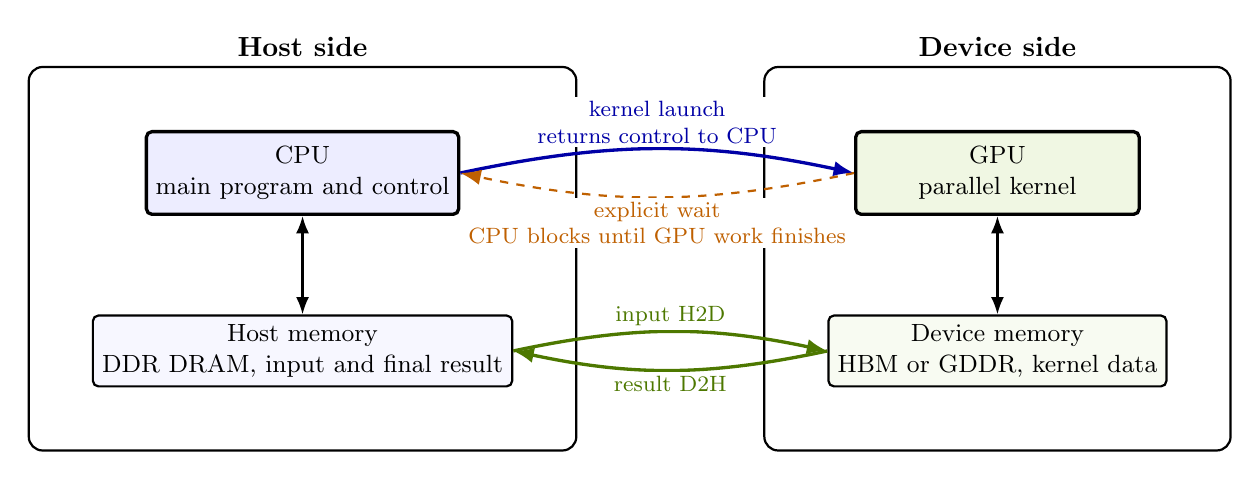
\begin{tikzpicture}[
    font=\small,
    processor/.style={draw,very thick,rounded corners=2pt,minimum width=3.6cm,
      minimum height=1.05cm,align=center},
    memory/.style={draw,thick,rounded corners=2pt,minimum width=3.6cm,
      minimum height=0.9cm,align=center},
    enclosure/.style={draw,thick,rounded corners=5pt,inner sep=8mm},
    control/.style={-{Latex[length=2.6mm]},very thick,blue!65!black},
    dataflow/.style={-{Latex[length=2.6mm]},very thick,nvidiagreen!65!black},
    completion/.style={-{Latex[length=2.6mm]},thick,dashed,orange!75!black},
    note/.style={align=center,font=\footnotesize,fill=white,inner sep=1.5pt}
  ]
    \node[processor,fill=blue!7] (cpu) {CPU\\main program and control};
    \node[memory,fill=blue!3,below=1.25cm of cpu] (hostmem)
      {Host memory\\DDR DRAM, input and final result};
    \node[processor,fill=nvidiagreen!11,right=5.0cm of cpu] (gpu) {GPU\\parallel kernel};
    \node[memory,fill=nvidiagreen!5,below=1.25cm of gpu] (devmem)
      {Device memory\\HBM or GDDR, kernel data};

    \node[enclosure,fit=(cpu)(hostmem),label={[font=\bfseries]above:Host side}] (host) {};
    \node[enclosure,fit=(gpu)(devmem),label={[font=\bfseries]above:Device side}] (device) {};

    \draw[control] (cpu.east) to[bend left=12]
      node[note,above] {kernel launch\\returns control to CPU} (gpu.west);
    \draw[completion] (gpu.west) to[bend left=12]
      node[note,below] {explicit wait\\CPU blocks until GPU work finishes} (cpu.east);
    \draw[dataflow] (hostmem.east) to[bend left=12]
      node[note,above] {input H2D} (devmem.west);
    \draw[dataflow] (devmem.west) to[bend left=12]
      node[note,below] {result D2H} (hostmem.east);

    \draw[{Latex[length=2.2mm]}-{Latex[length=2.2mm]},thick] (cpu) -- (hostmem);
    \draw[{Latex[length=2.2mm]}-{Latex[length=2.2mm]},thick] (devmem) -- (gpu);
  \end{tikzpicture}
  \caption{The CPU controls the program.  H2D and D2H mean host-to-device and
  device-to-host data movement.  A kernel launch returns control to the CPU; the CPU
  must later wait before reading the result.}
  \label{fig:cpu-gpu-interaction}
\end{figure}

The execution sequence is
\begin{enumerate}
  \item The CPU makes the input available to the GPU.
  \item The CPU launches the kernel and continues without waiting for the GPU.
  \item GPU threads compute the result.
  \item The CPU calls \code{cudaDeviceSynchronize()} and waits before reading the
  result.
\end{enumerate}

A simple time budget for a run with no overlap is
\begin{equation}
  T_{\mathrm{total}}
  =T_{\mathrm{host}}
   +T_{\mathrm{H2D}}
   +T_{\mathrm{launch}}
   +T_{\mathrm{kernel}}
   +T_{\mathrm{D2H}},
  \label{eq:heterogeneous-time-budget}
\end{equation}
$T_{\mathrm{host}}$ is CPU work outside the launch and copies.
$T_{\mathrm{H2D}}$ and $T_{\mathrm{D2H}}$ are the input and result copy times.
$T_{\mathrm{launch}}$ is the time the CPU spends submitting the kernel, and
$T_{\mathrm{kernel}}$ is the GPU execution time.  A later call to
\code{cudaDeviceSynchronize()} only makes the CPU wait for unfinished GPU work; it
does not add a second kernel execution.  Data rearrangement may add further terms.
If CPU work, copies, and kernel execution overlap, their times cannot simply be
added.

% ============================================================================
\subsection{Libraries and tools}
\label{chap:ecosystem}
% ============================================================================

Before writing a kernel, ask whether a tested implementation already exists.
\begin{equation}
  \text{application}
  \longrightarrow \text{numerical library}
  \longrightarrow \text{general CUDA building blocks}
  \longrightarrow \text{custom kernel}.
  \label{eq:abstraction-ladder}
\end{equation}
Use the leftmost level that provides the required operation and control.

Table~\ref{tab:cuda-scientific-libraries} maps common operations to CUDA
libraries~\cite{gupta2020ecosystem,cudax2026}.  NCCL is the NVIDIA Collective
Communications Library.
\begin{table}[ht!]
  \centering
  \caption{Common numerical operations and CUDA libraries.}
  \label{tab:cuda-scientific-libraries}
  \small
  \renewcommand{\arraystretch}{1.05}
  \begin{tabularx}{\textwidth}{@{}l l Y Y@{}}
    \toprule
    Mathematical task & Library & Physics example & Machine-learning example \\
    \midrule
    Dense matrix products & cuBLAS & basis changes, dense Hamiltonians
      & linear layers, batched general matrix multiplication \\
    Dense solvers & cuSOLVER & least squares, eigensystems
      & principal component analysis, linear regression \\
    Sparse algebra & cuSPARSE & sparse partial differential equation systems
      & graph neural networks, sparse features \\
    Fourier transforms & cuFFT & spectral methods, structure factors
      & spectral convolution, signal features \\
    Pseudorandom sampling & cuRAND & Monte Carlo and stochastic dynamics
      & initialization, dropout, sampling \\
    Tensor contractions & cuTENSOR & many-body tensor algebra
      & attention, \code{einsum} layers \\
    Collectives & NCCL & multi-GPU reductions
      & gradient all-reduce \\
    Partitioned global memory & NVSHMEM & fine-grained multi-GPU exchange
      & model and tensor parallelism \\
    \bottomrule
  \end{tabularx}
\end{table}

Before using a CUDA library, check how the library stores arrays, which numerical
precision the library uses, and whether the library applies any normalization.
Also check whether repeated calls with the same input must return the same result.

Choose the tool by what you need to see.
\begin{itemize}
  \item Nsight Systems shows the CPU and GPU timeline~\cite{nsightsystems2026}.
  \item Nsight Compute analyzes one GPU kernel~\cite{nsightcompute2026}.
  \item Compute Sanitizer detects memory-access and synchronization
  errors~\cite{computesanitizer2026}.
\end{itemize}

% ============================================================================
\Needspace{12\baselineskip}
\subsection{Programming model}
\label{chap:model}
% ============================================================================

At launch, the software defines a \emph{grid} of \emph{blocks} and \emph{threads}.
For example, \code{kernel<<<6, 64>>>(arguments)} creates one grid with six blocks
and 64 threads per block.  Every thread runs the kernel body.  The launch does not
name an SM.

The streaming multiprocessor (SM) is physical hardware.  CUDA assigns each whole
block to one SM, where it normally remains until it finishes.  Several blocks can
share an SM if resources permit.  The SM divides each block into consecutive groups
of 32 threads called \emph{warps}.  A warp is a scheduling group formed by the
hardware, not an object named in the launch or a fixed component inside the
SM~\cite{cuda-programming-guide}.

One A100 SM can keep at most $2{,}048$ threads, or 64 warps, resident.  One RTX 3090
SM can keep at most $1{,}536$ threads, or 48 warps, resident
\cite{cuda-programming-guide}.  Resident means that the thread's block is on the SM
and has not finished.  These numbers are capacity limits, not counts of arithmetic
units.  Register and shared-memory use can reduce them.

To keep the GPU busy, the program must launch enough blocks.  Too few blocks leaves
some SMs unused.  Each active SM also needs enough resident warps to run another
warp while one waits.  The program chooses the grid and block sizes; CUDA chooses
which SM runs each block.  Figure~\ref{fig:cuda-programming-model} shows this
mapping.

\begin{figure}[htbp]
  \centering
  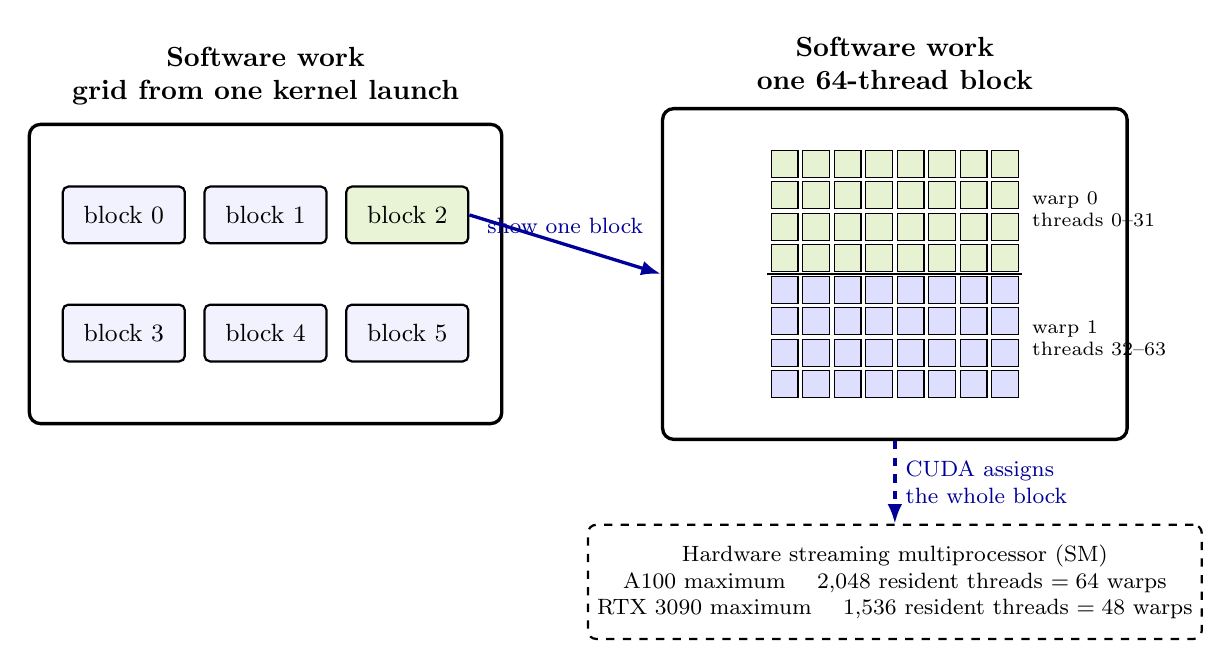
\begin{tikzpicture}[
    font=\small,
    gridbox/.style={draw,very thick,rounded corners=4pt,minimum width=6.0cm,
      minimum height=3.8cm},
    block/.style={draw,thick,rounded corners=2pt,minimum width=1.55cm,
      minimum height=0.72cm,align=center},
    detail/.style={draw,very thick,rounded corners=4pt,minimum width=5.9cm,
      minimum height=4.2cm},
    thread/.style={draw,fill=nvidiagreen!18,minimum size=0.34cm,inner sep=0pt},
    sm/.style={draw,thick,dashed,rounded corners=3pt,minimum width=6.5cm,
      minimum height=1.45cm,align=center,font=\footnotesize},
    map/.style={-{Latex[length=2.5mm]},very thick,blue!60!black}
  ]
    \node[gridbox] (grid) at (0,0) {};
    \node[font=\bfseries,align=center,above=1mm of grid.north]
      {Software work\\grid from one kernel launch};
    \node[block,fill=blue!5] at ($(grid.center)+(-1.8,0.75)$) {block 0};
    \node[block,fill=blue!5] at ($(grid.center)+(0,0.75)$) {block 1};
    \node[block,fill=nvidiagreen!16] (chosen) at ($(grid.center)+(1.8,0.75)$) {block 2};
    \node[block,fill=blue!5] at ($(grid.center)+(-1.8,-0.75)$) {block 3};
    \node[block,fill=blue!5] at ($(grid.center)+(0,-0.75)$) {block 4};
    \node[block,fill=blue!5] at ($(grid.center)+(1.8,-0.75)$) {block 5};

    \node[detail,right=2.0cm of grid] (detail) {};
    \node[font=\bfseries,align=center,above=1mm of detail.north]
      {Software work\\one 64-thread block};
    \foreach \x in {0,...,7}
      \foreach \y in {0,...,7} {
        \ifnum\y<4
          \node[thread,fill=nvidiagreen!18]
            at ($(detail.center)+({(\x-3.5)*0.40},{(3.5-\y)*0.40})$) {};
        \else
          \node[thread,fill=blue!13]
            at ($(detail.center)+({(\x-3.5)*0.40},{(3.5-\y)*0.40})$) {};
        \fi
      }
    \draw[thick] ($(detail.center)+(-1.62,0)$) -- ($(detail.center)+(1.62,0)$);
    \node[font=\scriptsize,anchor=west,align=left]
      at ($(detail.center)+(1.62,0.82)$)
      {warp 0\\threads 0--31};
    \node[font=\scriptsize,anchor=west,align=left]
      at ($(detail.center)+(1.62,-0.82)$)
      {warp 1\\threads 32--63};

    \node[sm,below=1.05cm of detail] (sm)
      {Hardware streaming multiprocessor (SM)\\
       A100 maximum \quad $2{,}048$ resident threads $=64$ warps\\
       RTX 3090 maximum \quad $1{,}536$ resident threads $=48$ warps};
    \draw[map] (chosen.east) -- node[above,font=\footnotesize] {show one block} (detail.west);
    \draw[map,dashed] (detail.south) --
      node[right,font=\footnotesize,align=left] {CUDA assigns\\the whole block} (sm.north);
  \end{tikzpicture}
  \caption{Software defines the grid, blocks, and threads.  CUDA assigns a whole
  block to an SM.  This 64-thread block becomes two 32-thread
  warps~\cite{gupta2020model,cuda-programming-guide}.}
  \label{fig:cuda-programming-model}
\end{figure}

\FloatBarrier

\Needspace{31\baselineskip}
A CUDA \emph{stream} belongs to one CUDA program.  It is a sequence of kernel
launches and memory operations that run in submission order
\cite{cuda-programming-guide}.  A launch that does not name a stream uses the
default stream.  For example, let \code{kernel\_1} and \code{kernel\_2} stand for
any two kernels.

\begin{lstlisting}[language=CUDA,numbers=none]
// Both kernels are submitted to the default stream.
kernel_1<<<grid, block>>>();
kernel_2<<<grid, block>>>();
\end{lstlisting}

The CPU can submit both launches without waiting.  On the GPU, however,
\code{kernel\_1} finishes before \code{kernel\_2} starts because both belong to the
same stream.

One program can instead create two streams and place one kernel in each.

\begin{lstlisting}[language=CUDA,numbers=none]
cudaStream_t stream_1, stream_2;
cudaStreamCreate(&stream_1);
cudaStreamCreate(&stream_2);

// The fourth launch argument selects the stream.
kernel_1<<<grid, block, 0, stream_1>>>();
kernel_2<<<grid, block, 0, stream_2>>>();
\end{lstlisting}

The third launch argument, zero, requests no dynamic shared memory.  The CPU again
submits both launches without waiting.  If the kernels are independent and the GPU
has enough free resources, their execution may overlap.  CUDA does not guarantee
overlap.

Two separate operating-system programs are not two CUDA streams.  They are separate
programs competing for the same GPU.  The example above uses two streams inside one
program to request concurrent kernel execution.

For a one-dimensional launch, a thread's global index is
\begin{equation}
  i=b_xB_x+t_x,
  \label{eq:chapter-global-index-1d}
\end{equation}
where $t_x=\code{threadIdx.x}$, $b_x=\code{blockIdx.x}$, and
$B_x=\code{blockDim.x}$.  Figure~\ref{fig:cuda-index-1d} shows a concrete
example.

\begin{figure}[htbp]
  \centering
  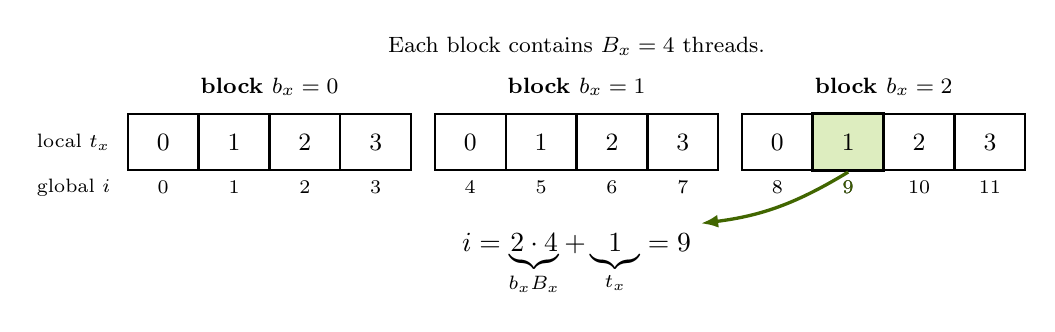
\begin{tikzpicture}[
    font=\small,
    threadcell/.style={draw,thick,minimum width=0.9cm,minimum height=0.72cm,
      inner sep=0pt},
    selectedcell/.style={threadcell,very thick,fill=nvidiagreen!25}
  ]
    \node[font=\footnotesize] at (5.25,1.22)
      {Each block contains $B_x=4$ threads.};
    \foreach \b in {0,...,2} {
      \pgfmathsetmacro{\xbase}{3.9*\b}
      \node[font=\footnotesize\bfseries] at ({\xbase+1.35},0.70)
        {block $b_x=\b$};
      \foreach \t in {0,...,3} {
        \pgfmathtruncatemacro{\globalindex}{4*\b+\t}
        \node[threadcell] at ({\xbase+0.9*\t},0) {$\t$};
        \node[font=\scriptsize] at ({\xbase+0.9*\t},-0.58)
          {$\globalindex$};
      }
    }
    \node[selectedcell] (chosen1d) at ({2*3.9+0.9},0) {$1$};
    \node[font=\scriptsize\bfseries,nvidiagreen!50!black]
      at ({2*3.9+0.9},-0.58) {$9$};
    \node[font=\scriptsize,anchor=east] at (-0.55,0) {local $t_x$};
    \node[font=\scriptsize,anchor=east] at (-0.55,-0.58) {global $i$};
    \node[font=\normalsize] (calc1d) at (5.25,-1.55)
      {$i=\underbrace{2\cdot4}_{b_xB_x}+\underbrace{1}_{t_x}=9$};
    \draw[-{Latex[length=2.2mm]},very thick,nvidiagreen!55!black]
      (chosen1d.south) to[bend left=12] (calc1d.north east);
  \end{tikzpicture}
  \caption{One-dimensional indexing.  Thread $t_x=1$ in block $b_x=2$ has
  global index $i=2\cdot4+1=9$.}
  \label{fig:cuda-index-1d}
\end{figure}

\FloatBarrier

In two dimensions,
\begin{align}
  i &= b_xB_x+t_x, \\
  j &= b_yB_y+t_y.
  \label{eq:chapter-global-index-2d}
\end{align}
Suppose the array stores all of row 0, then all of row 1, and so on.  This is called
\emph{row-major storage}.  If each row has $N_x$ columns, the one-dimensional index
is
\begin{equation}
  \ell=jN_x+i.
  \label{eq:row-major-index}
\end{equation}
Figure~\ref{fig:cuda-index-2d} shows both steps.  First obtain $(i,j)$ from the
block and thread coordinates, then convert $(i,j)$ to one index $\ell$.

\begin{figure}[htbp]
  \centering
  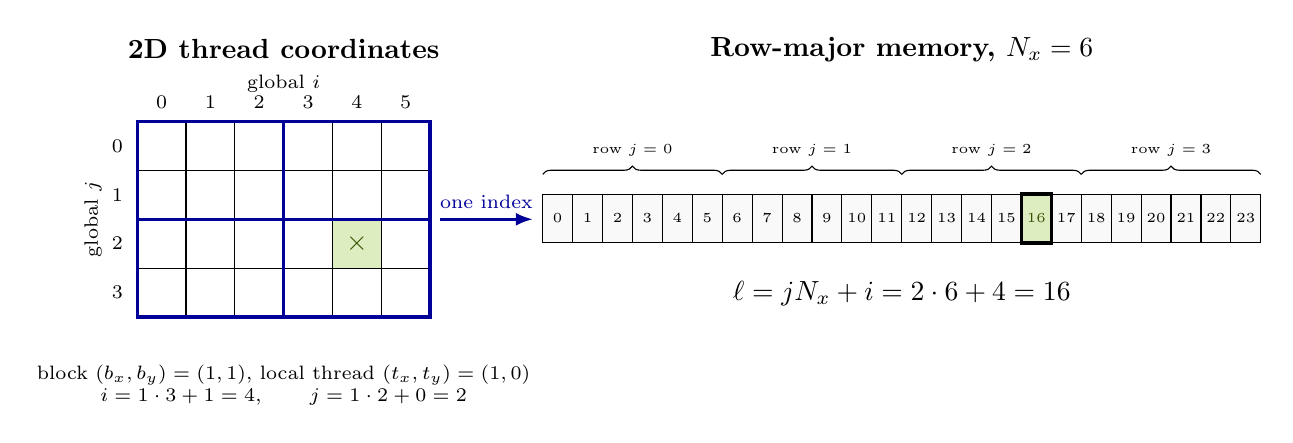
\begin{tikzpicture}[font=\small]
    \def\gridcell{0.62}
    \def\memcell{0.38}
    \def\memstart{5.15}

    \node[font=\bfseries] at ({3*\gridcell},0.92)
      {2D thread coordinates};
    \fill[nvidiagreen!25]
      ({4*\gridcell},{-2*\gridcell}) rectangle
      ({5*\gridcell},{-3*\gridcell});
    \foreach \x in {0,...,6}
      \draw[thin] ({\x*\gridcell},0) -- ({\x*\gridcell},{-4*\gridcell});
    \foreach \y in {0,...,4}
      \draw[thin] (0,{-\y*\gridcell}) -- ({6*\gridcell},{-\y*\gridcell});
    \foreach \bx in {0,1}
      \foreach \by in {0,1}
        \draw[very thick,blue!60!black]
          ({3*\bx*\gridcell},{-2*\by*\gridcell}) rectangle
          ({3*(\bx+1)*\gridcell},{-2*(\by+1)*\gridcell});
    \foreach \i in {0,...,5}
      \node[font=\scriptsize] at ({(\i+0.5)*\gridcell},0.25) {$\i$};
    \foreach \j in {0,...,3}
      \node[font=\scriptsize] at (-0.25,{-(\j+0.5)*\gridcell}) {$\j$};
    \node[font=\scriptsize] at ({3*\gridcell},0.48) {global $i$};
    \node[font=\scriptsize,rotate=90] at (-0.56,{-2*\gridcell}) {global $j$};
    \node[font=\bfseries,nvidiagreen!45!black]
      (chosen2d) at ({4.5*\gridcell},{-2.5*\gridcell}) {$\times$};
    \node[align=center,font=\scriptsize] at ({3*\gridcell},-3.35)
      {block $(b_x,b_y)=(1,1)$, local thread $(t_x,t_y)=(1,0)$\\
       $i=1\cdot3+1=4,\qquad j=1\cdot2+0=2$};

    \node[font=\bfseries] at ({\memstart+12*\memcell},0.92)
      {Row-major memory, $N_x=6$};
    \foreach \address in {0,...,23} {
      \pgfmathsetmacro{\xaddress}{\memstart+\address*\memcell}
      \draw[fill=gray!5]
        (\xaddress,-0.92) rectangle ({\xaddress+\memcell},-1.54);
      \node[font=\tiny] at ({\xaddress+0.5*\memcell},-1.23)
        {$\address$};
    }
    \foreach \row in {0,...,3} {
      \pgfmathsetmacro{\rowstart}{\memstart+6*\row*\memcell}
      \pgfmathsetmacro{\rowend}{\memstart+6*(\row+1)*\memcell}
      \draw[decorate,decoration={brace,amplitude=3pt}]
        (\rowstart,-0.67) -- (\rowend,-0.67)
        node[midway,above=3pt,font=\tiny] {row $j=\row$};
    }
    \pgfmathsetmacro{\selectedaddress}{\memstart+16*\memcell}
    \draw[very thick,fill=nvidiagreen!25]
      (\selectedaddress,-0.92) rectangle
      ({\selectedaddress+\memcell},-1.54);
    \node[font=\tiny\bfseries,nvidiagreen!45!black] (linear16)
      at ({\selectedaddress+0.5*\memcell},-1.23) {$16$};
    \draw[-{Latex[length=2.2mm]},very thick,blue!60!black]
      ({6*\gridcell+0.12},{-2*\gridcell}) --
      node[above,font=\scriptsize] {one index}
      ({\memstart-0.12},{-2*\gridcell});
    \node[font=\normalsize] at ({\memstart+12*\memcell},-2.18)
      {$\ell=jN_x+i=2\cdot6+4=16$};
  \end{tikzpicture}
  \caption{Two-dimensional indexing followed by row-major flattening.  The
  highlighted thread has array coordinate $(i,j)=(4,2)$ and linear index
  $\ell=16$.}
  \label{fig:cuda-index-2d}
\end{figure}

\FloatBarrier
Threads in the same block can exchange data through shared memory.
\code{\_\_syncthreads()} synchronizes those threads.  No thread continues past the
barrier until every thread in the block reaches it.  CUDA may start different
blocks in any order or run them on different SMs, so this barrier cannot
synchronize different blocks~\cite{cuda-memory-model}.

CUDA provides several places to store data.  The locations differ in capacity,
which threads can use them, and how long the data remains available.  L1 and L2
mean level-1 and level-2 cache.  Table~\ref{tab:memory-hierarchy} summarizes the
storage locations.
\begin{table}[htbp]
  \centering
  \caption{Where CUDA data can be stored and which threads can use it.}
  \label{tab:memory-hierarchy}
  \small
  \begin{tabularx}{\textwidth}{@{}>{\raggedright\arraybackslash}p{0.16\textwidth}
    >{\raggedright\arraybackslash}p{0.22\textwidth}
    >{\raggedright\arraybackslash}p{0.15\textwidth}Y@{}}
    \toprule
    Storage & Which threads can use it & How long it exists & What it is \\
    \midrule
    Registers & one thread & thread & fast storage inside the SM; limited amount \\
    Local memory & one thread & thread & private data stored in device memory \\
    Shared memory & one block & block & on-chip memory used explicitly by the kernel \\
    L1 cache & threads using one SM & managed by hardware & cache used by one SM \\
    L2 cache & all SMs on a device & managed by hardware & cache used by all SMs \\
    Global memory & all threads on a device & until freed & large device DRAM \\
    Host memory & CPU, and GPU when mapped or managed & until freed & system DRAM
      reached through the connection between CPU and GPU \\
    \bottomrule
  \end{tabularx}
\end{table}

Capacity tells us how much data fits in each memory level.  Performance also depends
on how often data moves between levels.  Shared memory is useful when threads reuse
values loaded once.  Without reuse, copying data through shared memory adds work but
does not reduce the bytes moved to and from global memory.

Compute capability identifies the CUDA features and resource limits supported by a
GPU.  It is not a speed rating.  A benchmark should therefore report the GPU model,
not only the compute capability~\cite{cuda-programming-guide}.

% ============================================================================
\subsection{Ampere A100 and RTX 3090}
\label{sec:ampere-comparison}
% ============================================================================

The A100 uses the Ampere GA100 chip, while the RTX 3090 uses GA102.  Both follow
the same CUDA execution model but differ in arithmetic throughput and memory
\cite{ampere2020,ga102whitepaper}.

The architecture diagrams show the complete chips, not the product configurations.
Figure~\ref{fig:ga100-full-gpu} shows all 128 SMs in GA100; the A100 enables 108.
GA102 contains 84 SMs, while the RTX 3090 enables 82
\cite{ampere2020,ga102whitepaper,rtx3090specs}.

\begin{figure}[htbp]
  \centering
  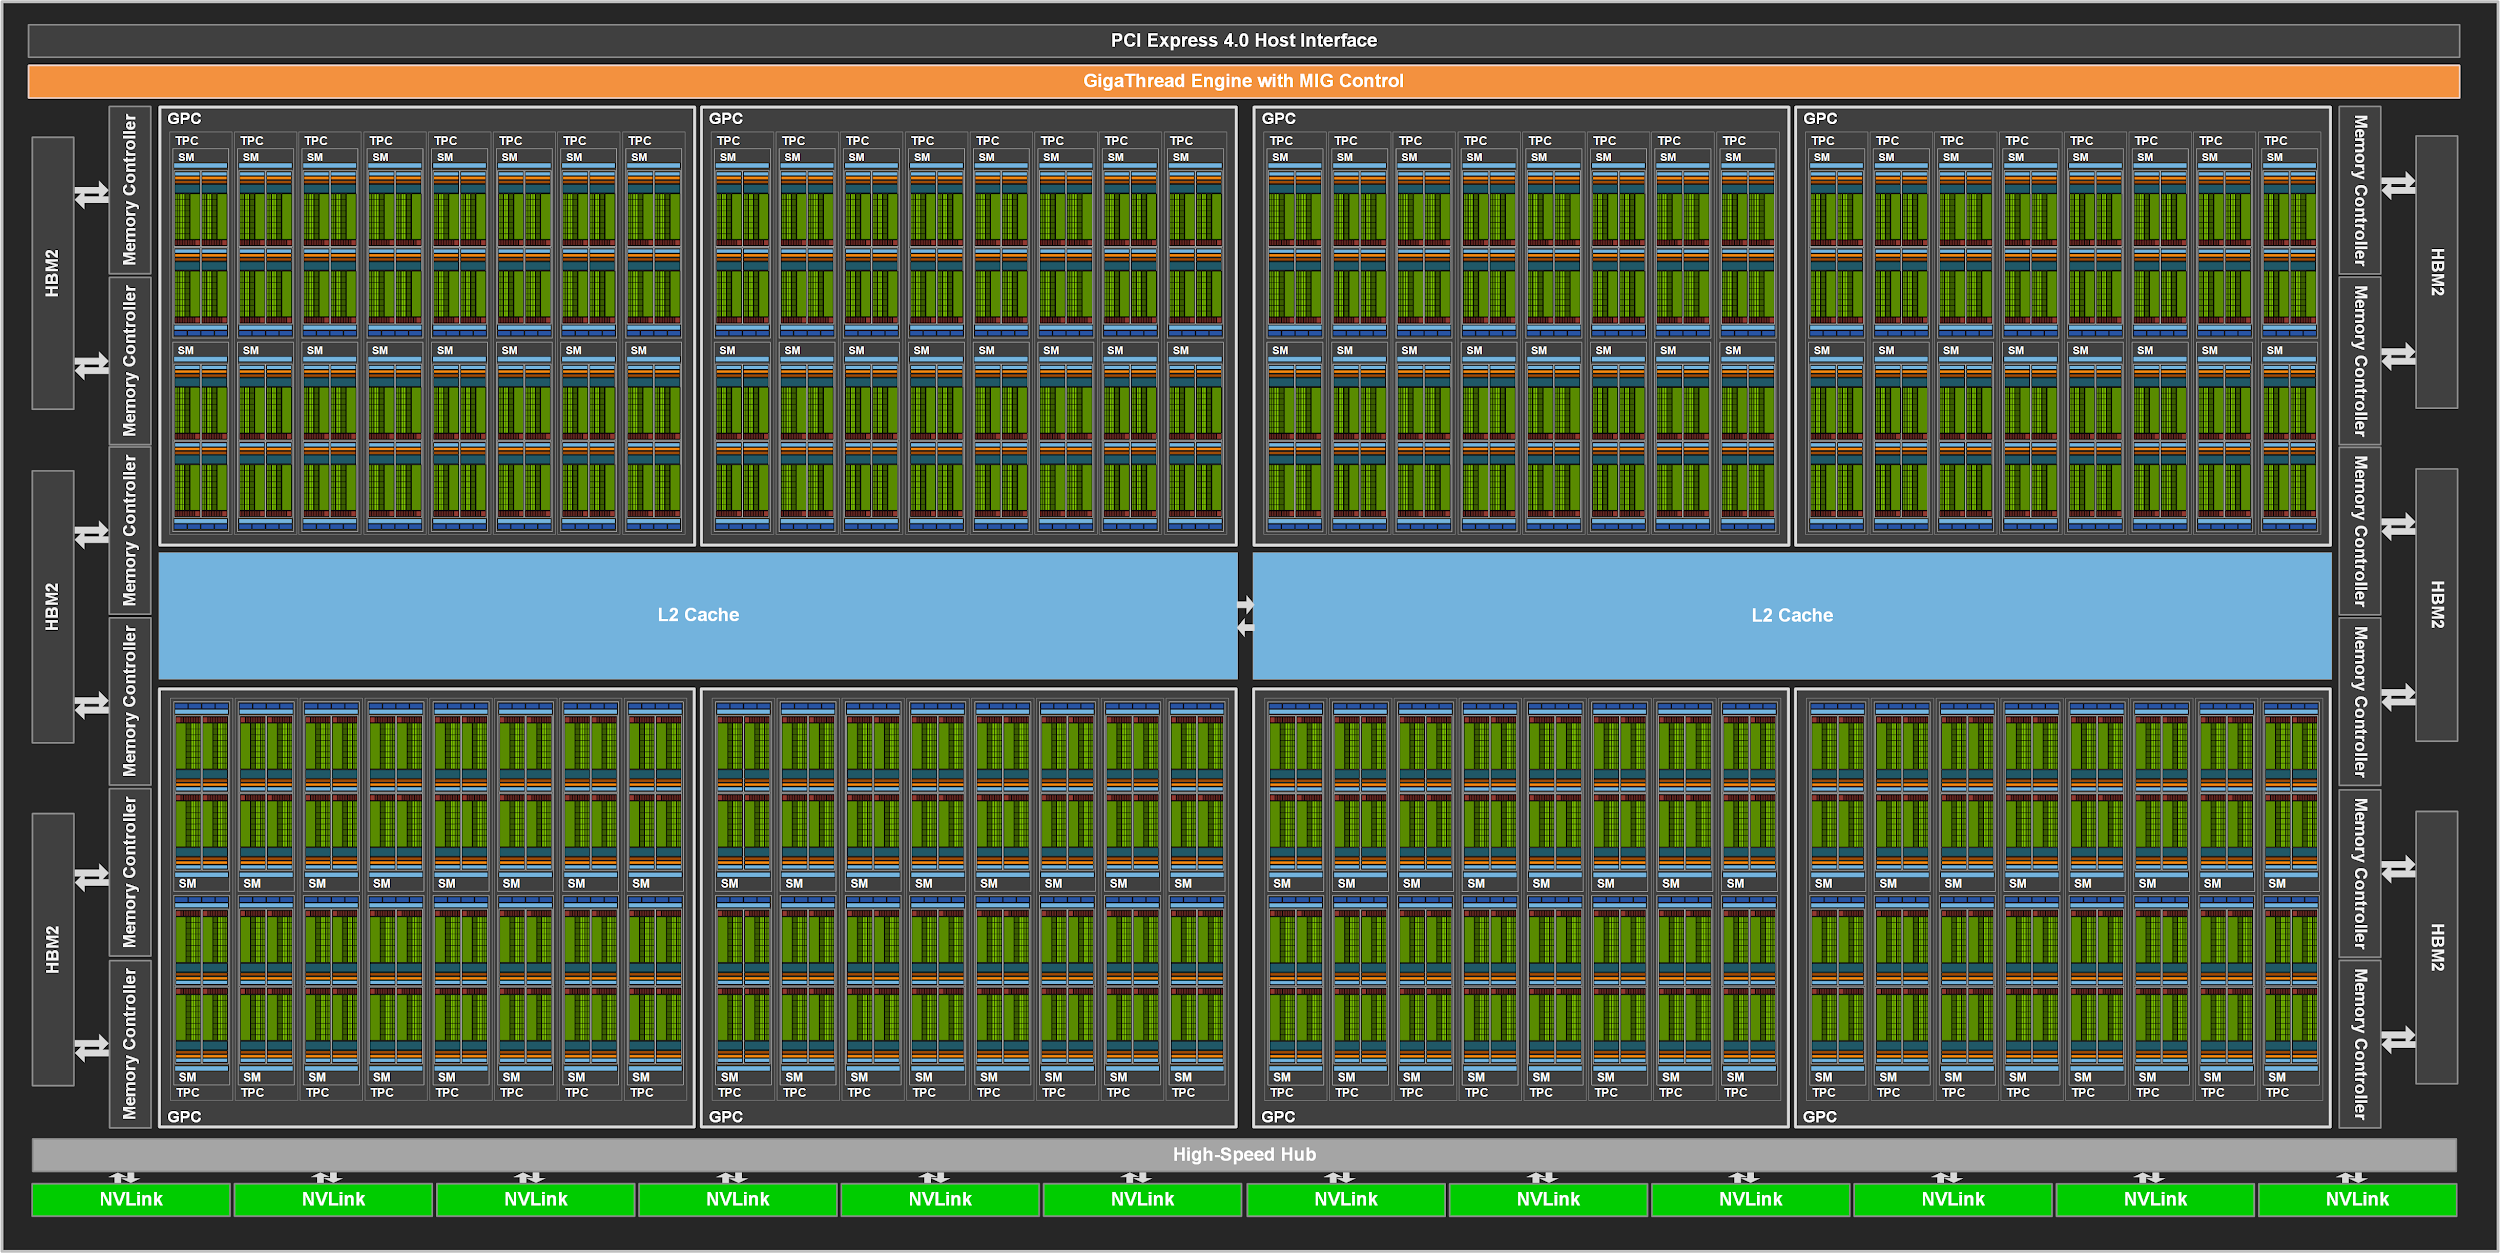
\includegraphics[width=\textwidth]{figures/nvidia-ga100-full-gpu.png}
  \caption{Complete GA100 chip design.  Reproduced from
  NVIDIA~\cite{ampere2020}.}
  \label{fig:ga100-full-gpu}
\end{figure}

Figure~\ref{fig:ga100-sm} shows one GA100 SM.  Its four sections share the L1 cache
and shared memory.  A block remains on the SM while its warps run there.

\begin{figure}[htbp]
  \centering
  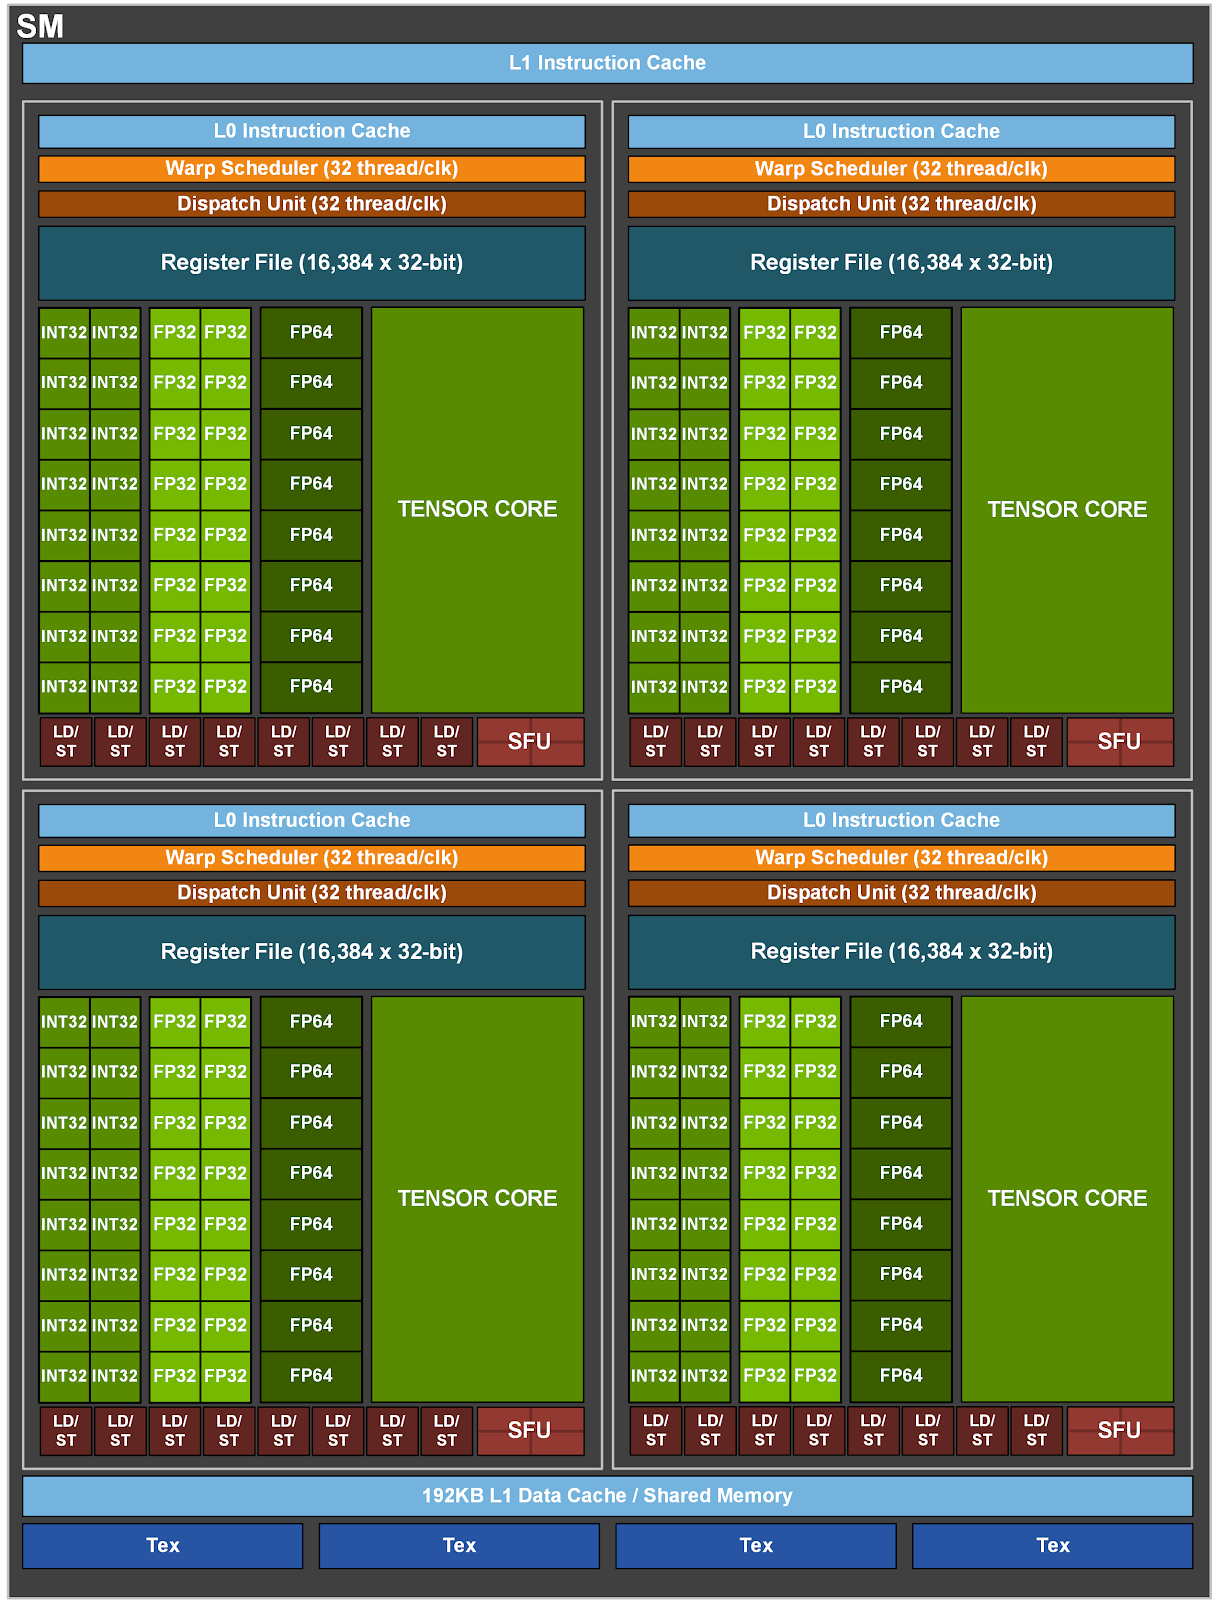
\includegraphics[width=0.74\textwidth]{figures/nvidia-ga100-sm.png}
  \caption{One GA100 streaming multiprocessor.  Reproduced from
  NVIDIA~\cite{ampere2020}.}
  \label{fig:ga100-sm}
\end{figure}
\FloatBarrier

Table~\ref{tab:a100-3090} compares 32-bit floating-point (FP32) throughput, 64-bit
floating-point (FP64) throughput, device-memory capacity, memory bandwidth, and the
maximum number of resident threads per SM.  Throughput is given in tera
floating-point operations per second (TFLOP/s).  The devices use High Bandwidth
Memory 2 (HBM2) and Graphics Double Data Rate 6X (GDDR6X) memory
\cite{ampere2020,ga102whitepaper,rtx3090specs,cuda-programming-guide}.

\begin{table}[htbp]
  \centering
  \small
  \caption{Selected specifications for two Ampere GPUs
  \cite{ampere2020,ga102whitepaper,rtx3090specs,cuda-programming-guide}.}
  \label{tab:a100-3090}
  \begin{tabularx}{\textwidth}{@{}>{\raggedright\arraybackslash}p{0.22\textwidth}YY@{}}
    \toprule
    & A100 40 GB (GA100) & RTX 3090 (GA102) \\
    \midrule
    FP32 throughput
      & $19.5\ \mathrm{TFLOP/s}$
      & $35.6\ \mathrm{TFLOP/s}$ \\
    FP64 throughput
      & $9.7\ \mathrm{TFLOP/s}$
      & $0.56\ \mathrm{TFLOP/s}$ \\
    Device memory
      & $40\ \mathrm{GB}$ HBM2, $1555\ \mathrm{GB/s}$
      & $24\ \mathrm{GB}$ GDDR6X, $936\ \mathrm{GB/s}$ \\
    Maximum resident threads per SM
      & $2{,}048$
      & $1{,}536$ \\
    \bottomrule
  \end{tabularx}
\end{table}
\FloatBarrier

The throughput and bandwidth entries are vendor peak values, not measurements from
the example programs.  GA102 FP64 throughput is $1/64$ of its FP32 throughput, so
the RTX 3090 value is $35.6/64=0.56\ \mathrm{TFLOP/s}$ after
rounding~\cite{ga102whitepaper}.

\newpage
\section{Array addition}

\subsection{Vector addition}
\label{chap:vector-add}

Let \(x\) and \(y\) be arrays of \(N=2^{20}\) floating-point numbers.  The program
adds \(x\) to \(y\):
\begin{equation}
  y_i \leftarrow x_i+y_i,
  \qquad i=0,\ldots,N-1.
  \label{eq:vector-add}
\end{equation}
If every \(x_i=1\) and every \(y_i=2\) before the addition, every output should be
3.  The CPU version is one loop.
\begin{lstlisting}[language=C++,caption={Serial CPU addition.}]
void add_cpu(int n, const float* x, float* y) {
  // One CPU thread processes the array from beginning to end.
  for (int i = 0; i < n; ++i) {
    y[i] = x[i] + y[i];
  }
}
\end{lstlisting}

A CUDA kernel is a function that runs on the GPU.  The CPU launches a kernel with
\code{<<<number\_of\_blocks, threads\_per\_block>>>}.  The simplest launch uses one
GPU thread, so that thread repeats the CPU loop.
\begin{lstlisting}[language=CUDA,caption={One GPU thread processes the whole array.}]
__global__ void add_one_thread(int n, const float* x, float* y) {
  // This loop is serial because the launch below creates only one GPU thread.
  for (int i = 0; i < n; ++i) {
    y[i] = x[i] + y[i];
  }
}

// CPU code: launch one block containing one thread.
add_one_thread<<<1, 1>>>(N, x, y);
\end{lstlisting}

To use many threads, give each thread a different first array index.  The first line
of \code{add\_grid} is Equation~\eqref{eq:chapter-global-index-1d} from
Section~\ref{chap:model}.
\begin{lstlisting}[language=CUDA,caption={Many GPU threads divide the array.}]
__global__ void add_grid(int n, const float* x, float* y) {
  // This thread begins at one distinct array index.
  const int index = blockIdx.x * blockDim.x + threadIdx.x;
  // This is the total number of threads created by the launch.
  const int stride = blockDim.x * gridDim.x;

  // If needed, this thread continues one complete grid farther in the array.
  for (int i = index; i < n; i += stride) {
    y[i] = x[i] + y[i];
  }
}
\end{lstlisting}

The CPU chooses 256 threads per block and creates enough blocks to cover the array.
\begin{lstlisting}[language=CUDA]
const int threads_per_block = 256;
const int number_of_blocks =
    (N + threads_per_block - 1) / threads_per_block;

// CPU code: launch the parallel kernel on the GPU.
add_grid<<<number_of_blocks, threads_per_block>>>(N, x, y);

// Wait before the CPU checks the result.
cudaDeviceSynchronize();
\end{lstlisting}
C++ integer division discards the remainder, so adding
\code{threads\_per\_block - 1} rounds the number of blocks up.  For \(N=1000\),
the launch creates \(4\times256=1024\) threads.  Threads 0 through 999 perform the
addition.  Threads 1000 through 1023 test \code{i < n}, find it false, make no array
access, and finish.  They are still real threads in the kernel launch; they simply
have no array element to process.

For the launch above, each valid thread processes one element.  The
\code{i += stride} update also lets the same kernel work with fewer threads: after
processing \(i\), a thread next processes \(i+\code{stride}\).

\paragraph{Unified Memory.}
The CPU and GPU normally use separate memory allocations.  Unified Memory creates
allocations that both can address through the same pointers.  This simplifies the
code, but the array data must still move between CPU memory and GPU memory.
Figure~\ref{fig:unified-memory} shows the difference.

\begin{figure}[htbp]
  \centering
  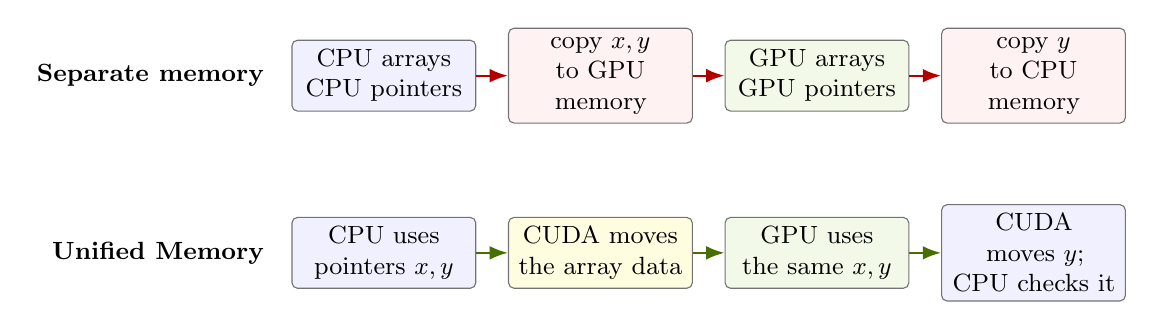
\begin{tikzpicture}[
    >=Latex,
    box/.style={draw=black!55,rounded corners=2pt,minimum height=0.9cm,
      text width=2.1cm,align=center,font=\small},
    copy/.style={->,red!70!black,thick},
    managed/.style={->,nvidiagreen!60!black,thick},
    rowlabel/.style={font=\small\bfseries,anchor=east},
  ]
    \node[rowlabel] at (-5.55,1.25) {Separate memory};
    \node[box,fill=blue!6] (host1) at (-4.15,1.25) {CPU arrays\\CPU pointers};
    \node[box,fill=red!5] (copy1) at (-1.4,1.25) {copy \(x,y\)\\to GPU memory};
    \node[box,fill=nvidiagreen!9] (gpu1) at (1.35,1.25) {GPU arrays\\GPU pointers};
    \node[box,fill=red!5] (copy2) at (4.1,1.25) {copy \(y\)\\to CPU memory};
    \draw[copy] (host1) -- (copy1);
    \draw[copy] (copy1) -- (gpu1);
    \draw[copy] (gpu1) -- (copy2);

    \node[rowlabel] at (-5.55,-1.0) {Unified Memory};
    \node[box,fill=blue!6] (host2) at (-4.15,-1.0) {CPU uses\\pointers \(x,y\)};
    \node[box,fill=yellow!12] (move1) at (-1.4,-1.0) {CUDA moves\\the array data};
    \node[box,fill=nvidiagreen!9] (gpu2) at (1.35,-1.0) {GPU uses\\the same \(x,y\)};
    \node[box,fill=blue!6] (host3) at (4.1,-1.0) {CUDA moves \(y\);\\CPU checks it};
    \draw[managed] (host2) -- (move1);
    \draw[managed] (move1) -- (gpu2);
    \draw[managed] (gpu2) -- (host3);
  \end{tikzpicture}
  \caption{Unified Memory removes separate CPU and GPU pointers, not the data
  movement between CPU memory and GPU memory.}
  \label{fig:unified-memory}
\end{figure}

The essential allocation and use are:
\begin{lstlisting}[language=CUDA,basicstyle=\ttfamily\footnotesize]
float *x = nullptr, *y = nullptr;
const std::size_t bytes = N * sizeof(float);

// CUDA stores the two allocation addresses in x and y.
cudaMallocManaged(&x, bytes);
cudaMallocManaged(&y, bytes);

// CPU initializes x and y.
for (int i = 0; i < N; ++i) {
  x[i] = 1.0f;
  y[i] = 2.0f;
}

// GPU uses the same pointers.
add_grid<<<number_of_blocks, threads_per_block>>>(N, x, y);
cudaDeviceSynchronize();

// CPU can now check y.
cudaFree(x);
cudaFree(y);
\end{lstlisting}
Here \code{\&x} means the address of the pointer variable \code{x}.  CUDA needs
that address so it can store the allocation address in \code{x}.  The complete
program asks CUDA to move the input arrays to GPU memory before the kernel and move
the result back afterward.  This keeps the transfer time separate from the kernel
time in the profile; the allocation is still Unified Memory.

All runnable code and measurement records are in this repository:
\begin{center}
  \url{https://github.com/HaowuDuan/cuda-example-for-note}
\end{center}
From the repository root, build and run \path{add_grid.cu} with:
\begin{lstlisting}[language=bash,numbers=none]
# Compile the example, then run it.
nvcc -O3 -lineinfo add_grid.cu -o add_grid
./add_grid
\end{lstlisting}
The expected output is \code{Max error = 0}.  The \code{-lineinfo} option lets the
profiling tools connect their reports to source lines.

\subsection{Profiling}
\label{chap:profiling}

A kernel can be limited by data movement, arithmetic, or the cost of starting the
kernel.  The following kernel is a simple way to separate the three cases.
\begin{lstlisting}[language=CUDA,caption={One kernel used with different array and loop sizes.}]
__global__ void playground(float* data, int n, int repeats,
                           float multiplier, float offset) {
  // Give this thread one array element.
  const int index = blockIdx.x * blockDim.x + threadIdx.x;

  if (index < n) {
    // Load once, perform repeats updates, then store once.
    float value = data[index];
    for (int r = 0; r < repeats; ++r) {
      value = value * multiplier + offset;
    }
    data[index] = value;
  }
}
\end{lstlisting}

\begin{itemize}
  \item \textbf{Memory-bound.}  Use a large array and few arithmetic updates.
  The arithmetic finishes quickly, then compute waits for more data.

  \item \textbf{Compute-bound.}  Use a large \code{repeats} value.  The array
  element is already available while the arithmetic continues.  This is useful
  work if the updates are required; otherwise the kernel is simply doing
  unnecessary arithmetic.

  \item \textbf{Overhead-bound.}  Use a very small array and few updates.  The GPU
  finishes the work quickly, so the fixed cost of launching the kernel becomes a
  large part of the total time.
\end{itemize}

Splitting one calculation across many kernels can add another cost.  A value kept
inside one kernel may have to be written to GPU memory at the end of one kernel and
read again by the next.  This extra data movement is distinct from kernel launch
time.

The array-addition program demonstrates three CUDA tools.  Each answers one
question.

\paragraph{Compute Sanitizer: is the program accessing memory correctly?}
\begin{lstlisting}[language=bash,numbers=none]
# Check GPU memory accesses.
compute-sanitizer --tool memcheck ./add_grid
\end{lstlisting}
A correct run prints \code{Max error = 0} and ends with
\code{ERROR SUMMARY: 0 errors}~\cite{computesanitizer2026}.

\paragraph{Nsight Systems: where does the complete run spend time?}
\begin{lstlisting}[language=bash,numbers=none]
# Record CPU calls, data movement, and GPU work on one timeline.
nsys profile --trace=cuda --stats=true \
  --force-overwrite=true --output=add_grid_systems ./add_grid
\end{lstlisting}
The command saves \path{add_grid_systems.nsys-rep}.  Open that report in Nsight
Systems to see when the CPU submits work, when the arrays move, and when
\code{add\_grid} runs~\cite{nsightsystems2026}.

On the office RTX 3090, Nsight Systems measured 8.389~MB moving from CPU memory to
GPU memory, 4.194~MB moving back, and 15.072~\(\mu\mathrm{s}\) for
\code{add\_grid}.  The exact command, hardware, driver, and raw output are recorded
in \path{measurements/office_rtx3090_2026-09-01.txt} in the code repository.
One array contains \(2^{20}\) four-byte floats, so its size is 4.194~MB.  Two input
arrays move to the GPU and one result array moves back.

\paragraph{Nsight Compute: what limits the addition kernel?}
\begin{lstlisting}[language=bash,numbers=none]
# Inspect the launch, arithmetic use, and memory use of add_grid.
ncu --launch-count 1 \
  --section LaunchStats \
  --section SpeedOfLight \
  --section MemoryWorkloadAnalysis \
  --force-overwrite -o add_grid_compute ./add_grid
\end{lstlisting}
The three section names are Nsight Compute's names.  \code{LaunchStats} reports the
number of blocks and threads.  \code{SpeedOfLight} compares the kernel's arithmetic
and memory use with the GPU's measured limits.
\code{MemoryWorkloadAnalysis} reports the kernel's memory traffic
~\cite{nsightcompute2026,nsightcompute-profiling}.

Array addition reads \(x_i\), reads \(y_i\), and writes the new \(y_i\).  Since a
\code{float} occupies four bytes, the minimum traffic is \(12N\) bytes.  Its
effective bandwidth is therefore
\begin{equation}
  \mathcal{B}_{\mathrm{eff}}
  =\frac{12N}{t_{\mathrm{kernel}}}.
  \label{eq:effective-bandwidth}
\end{equation}
For \(N=2^{20}\) and the measured kernel time of 15.072~\(\mu\mathrm{s}\), this is
834.9~GB/s.  The kernel moves twelve bytes for one addition, so memory movement,
not arithmetic, is the main limit.
\newpage
\section{Performance limits and failure modes}
\label{sec:gpu-underutilization}
% ============================================================================

Section 2 separated three basic limits: data movement, arithmetic, and kernel
launch.  This section shows how those limits appear in code.  Every example follows
the same order: identify the problem, compare two implementations, explain the
difference, and state what to change.  One kernel can have more than one problem.

\begin{table}[htbp]
  \centering
  \small
  \caption{The question answered by each example.}
  \begin{tabularx}{\textwidth}{@{}>{\raggedright\arraybackslash}p{0.23\textwidth}YY@{}}
    \toprule
    \textbf{Problem} & \textbf{What happens} & \textbf{Main correction} \\
    \midrule
    Memory-bound kernel & Compute waits for array data & Remove unnecessary reads and writes \\
    Compute-bound kernel & Arithmetic takes most of the time & Remove unnecessary arithmetic \\
    Uncoalesced access & A warp needs many memory transactions & Give adjacent threads adjacent addresses \\
    Warp divergence & One warp runs both branches & Group threads that choose the same branch \\
    Atomic contention & Threads wait to update one value & Combine updates before the atomic operation \\
    Memory latency & Every resident warp is waiting & Keep enough warps available on each SM \\
    Launch overhead & The GPU waits for the next launch & Combine very small kernels \\
    CPU--GPU transfer & Copies take most of the time & Keep arrays in GPU memory \\
    \bottomrule
  \end{tabularx}
\end{table}

The source is in
\url{https://github.com/HaowuDuan/cuda-example-for-note}.  Each folder under
\path{failure_modes} contains \code{unoptimized.cu} and \code{optimized.cu}.
From the repository root, build all eight pairs and run one pair with:
\begin{lstlisting}[language=bash,numbers=none]
# Build every pair, then run the two transpose versions.
make -C failure_modes
./failure_modes/coalescing/unoptimized
./failure_modes/coalescing/optimized
\end{lstlisting}
Compare the two times on the same machine during the same session.  GPU clock,
temperature, driver, and other running programs can change the result.

% ----------------------------------------------------------------------------
\Needspace{15\baselineskip}
\subsection{Memory-bound kernels}
% ----------------------------------------------------------------------------

A kernel is \emph{memory-bound} when moving the input and output takes longer than
the arithmetic.  The arithmetic units then wait for data, and faster arithmetic
cannot reduce the running time.

Consider
\begin{equation}
  z_i=a(x_i+y_i).
  \label{eq:bandwidth-fusion-example}
\end{equation}
A two-kernel implementation first computes $t_i=x_i+y_i$, then computes
$z_i=a t_i$.  For single-precision arrays and ignoring the cache, the bytes moved are
\begin{itemize}
  \item $12N$ bytes for the first kernel, which reads $x$ and $y$ and writes $t$;
  \item $8N$ bytes for the second kernel, which reads $t$ and writes $z$.
\end{itemize}
The two kernels move $20N$ bytes in total.  A single kernel can read $x$ and $y$,
compute $a(x+y)$, and write $z$, moving only $12N$ bytes.  Both versions perform the
same arithmetic, but the single kernel never writes or reads the temporary array.
Combining the two operations is called \emph{kernel fusion}.
Figure~\ref{fig:bandwidth-fusion} shows the removed write and read.

\begin{figure}[htbp]
  \centering
  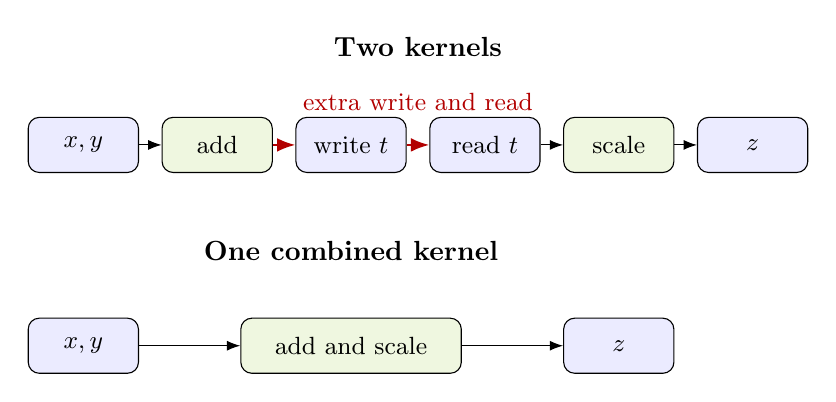
\begin{tikzpicture}[>=Latex,font=\small,
    box/.style={draw,rounded corners,minimum height=7mm,minimum width=14mm,align=center},
    mem/.style={box,fill=blue!8}, op/.style={box,fill=nvidiagreen!12}]
    \node[font=\bfseries] at (4.25,1.25) {Two kernels};
    \node[mem] (xy1) at (0,0) {$x,y$};
    \node[op] (add1) at (1.7,0) {add};
    \node[mem] (tmpw) at (3.4,0) {write $t$};
    \node[mem] (tmpr) at (5.1,0) {read $t$};
    \node[op] (scale1) at (6.8,0) {scale};
    \node[mem] (z1) at (8.5,0) {$z$};
    \draw[->] (xy1)--(add1);
    \draw[->,red!70!black,thick] (add1)--(tmpw);
    \draw[->,red!70!black,thick] (tmpw)--(tmpr);
    \draw[->] (tmpr)--(scale1);
    \draw[->] (scale1)--(z1);

    \node[font=\bfseries] at (3.4,-1.35) {One combined kernel};
    \node[mem] (xy2) at (0,-2.55) {$x,y$};
    \node[op,minimum width=28mm] (fused) at (3.4,-2.55) {add and scale};
    \node[mem] (z2) at (6.8,-2.55) {$z$};
    \draw[->] (xy2)--(fused);
    \draw[->] (fused)--(z2);
    \node[red!70!black] at (4.25,0.55) {extra write and read};
  \end{tikzpicture}
  \caption{One combined kernel removes the write and later read of the temporary
  array without changing the result.}
  \label{fig:bandwidth-fusion}
\end{figure}
\FloatBarrier

\textbf{What to change.}
Move less data.  Combine operations when doing so removes an intermediate array.
Reuse a value instead of writing it to GPU memory and reading it again.  Once memory
is already moving data as fast as it can, faster arithmetic will not help
\cite{cuda-best-practices,nsightcompute-profiling}.

% ----------------------------------------------------------------------------
\subsection{Compute-bound kernels}
% ----------------------------------------------------------------------------

A kernel is \emph{compute-bound} when the arithmetic takes longer than loading and
storing the data.  Being compute-bound is not a problem when every operation is
needed.  The kernel is wasteful only when the code repeats a calculation or uses a
needlessly expensive one.

For each input $x$, both supplied kernels evaluate the same degree-32 polynomial.
The coefficients are $a_p=10^{-3}(p+1)$ for $p=0,\ldots,32$.  The direct expression
and Horner's form are
\begin{equation}
  P(x)
  =\sum_{p=0}^{32}a_p x^p
  =a_0+x\bigl(a_1+x\bigl(a_2+\cdots+x(a_{31}+x a_{32})\bigr)\bigr).
  \label{eq:horner-form}
\end{equation}
The unoptimized kernel rebuilds every power $x^p$ from $1$.  Those loops perform
$\sum_{p=0}^{32}p=528$ multiplications, followed by 33 multiply-adds for the sum.
The Horner kernel starts with $r=a_{32}$ and applies $r\leftarrow rx+a_p$ for
$p=31,30,\ldots,0$.  It uses 32 multiply-adds and never constructs a power
separately.  The CUDA function \code{fmaf(u, v, w)} computes $uv+w$.

The chosen degree makes the difference easy to measure.  Both kernels still read
one float and write one float per element.  Horner's form changes the arithmetic
work without changing the bytes moved.

The roofline plot compares both examples with the GPU's memory and arithmetic
limits.  It is a reference, not a score.  Let $F$ be the number of floating-point
operations, $Q$ the minimum bytes read and written, and $T$ the measured time.
Arithmetic intensity $I$, measured performance $P$, and the roofline bound are
\begin{equation}
  I=\frac{F}{Q},
  \qquad
  P=\frac{F}{T},
  \qquad
  P_{\mathrm{roof}}(I)=\min\!\left(B_{\max}I,P_{\max}\right).
  \label{eq:roofline}
\end{equation}
Here $B_{\max}$ is peak device-memory bandwidth and $P_{\max}$ is peak arithmetic
throughput.  The diagonal part of the roof is the memory limit $B_{\max}I$.  The
horizontal part is the arithmetic limit $P_{\max}$
\cite{williams2009roofline}.

For the RTX 3090, Table~\ref{tab:a100-3090} gives
$B_{\max}=936\ \mathrm{GB/s}$ and $P_{\max}=35.6\ \mathrm{TFLOP/s}$.  The two
limits meet at
\[
  I=\frac{35.6\times10^{12}}{936\times10^9}
   =38.0\ \text{floating-point operations per byte}.
\]

Table~\ref{tab:roofline-measurements} gives the plotted measurements.  One
multiply-add counts as two floating-point operations.  Each program first performs
one warm-up.  The bandwidth programs report the mean of 20 launches and the
polynomial programs report the mean of 10.  The table uses the median of seven
program runs on the office RTX 3090.  The raw output and setup are in
\path{measurements/roofline_rtx3090_2026-09-01.txt} in the code repository
\cite{roofline-measurement}.

\begin{table}[htbp]
  \centering
  \small
  \caption{Measured coordinates for Figure~\ref{fig:measured-roofline}.}
  \label{tab:roofline-measurements}
  \begin{tabularx}{\textwidth}{@{}Yrrr@{}}
    \toprule
    \textbf{Implementation} &
      \textbf{FLOP/byte} &
      \textbf{Median time (ms)} &
      \textbf{GFLOP/s} \\
    \midrule
    Two kernels, $z=a(x+y)$ & $0.100$ & $0.400896$ & $83.7$ \\
    Fused kernel, $z=a(x+y)$ & $0.167$ & $0.239549$ & $140.1$ \\
    Direct polynomial powers & $74.25$ & $0.363389$ & $6856.1$ \\
    Horner's form & $8.00$ & $0.042474$ & $6320.0$ \\
    \bottomrule
  \end{tabularx}
\end{table}

\begin{figure}[htbp]
  \centering
  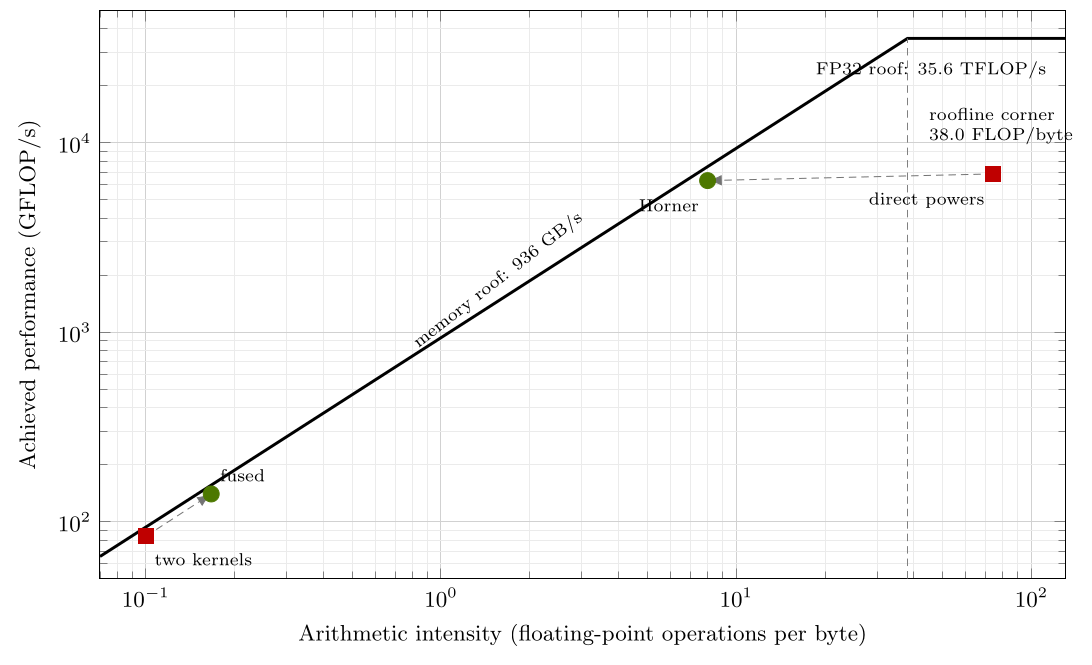
\includegraphics[width=0.94\textwidth]{figures/rtx3090-roofline.pdf}
  \caption{Roofline for the Section 3.1 and 3.2 examples on the RTX 3090.
  The black roof uses vendor peak values; the four points are measurements.
  Fusion moves the memory example up and to the right because it removes bytes.
  Horner's form moves the polynomial example left because it removes arithmetic.}
  \label{fig:measured-roofline}
\end{figure}
\FloatBarrier

The two memory points reach about $90\%$ of their bandwidth roof.  Fusion reduces
the time by a factor of $1.67$.  Horner's form reduces the polynomial time by a
factor of $8.56$.  Its plotted GFLOP/s is slightly lower because it performs far
fewer operations.  The roofline is an upper bound; it does not say that every
instruction sequence reaches the horizontal peak.

\Needspace{6\baselineskip}
\textbf{What to change.}
First remove arithmetic that does not change the answer.  If all the work is needed,
measure whether the arithmetic hardware is being used well.  Use lower precision
only when the required accuracy permits it.  For matrix operations, try a tested
library before writing a replacement kernel.

% ----------------------------------------------------------------------------
\Needspace{28\baselineskip}
\subsection{Uncoalesced memory access}
% ----------------------------------------------------------------------------

A warp contains 32 threads.  When those threads read or write adjacent floats, the
GPU can combine their work into a small number of memory transactions.  When their
addresses are far apart, the GPU needs more transactions to move the same 32
floats.  This slower pattern is called \emph{uncoalesced memory access}.

The example transposes a $4096\times4096$ matrix.  The program divides the matrix
into $32\times32$ square regions called \emph{tiles} and assigns one CUDA block to
each tile.  Figure~\ref{fig:transpose-tile-map} follows one tile from the matrix to
its block and then to one representative thread.

\begin{figure}[htbp]
  \centering
  \resizebox{\textwidth}{!}{%
  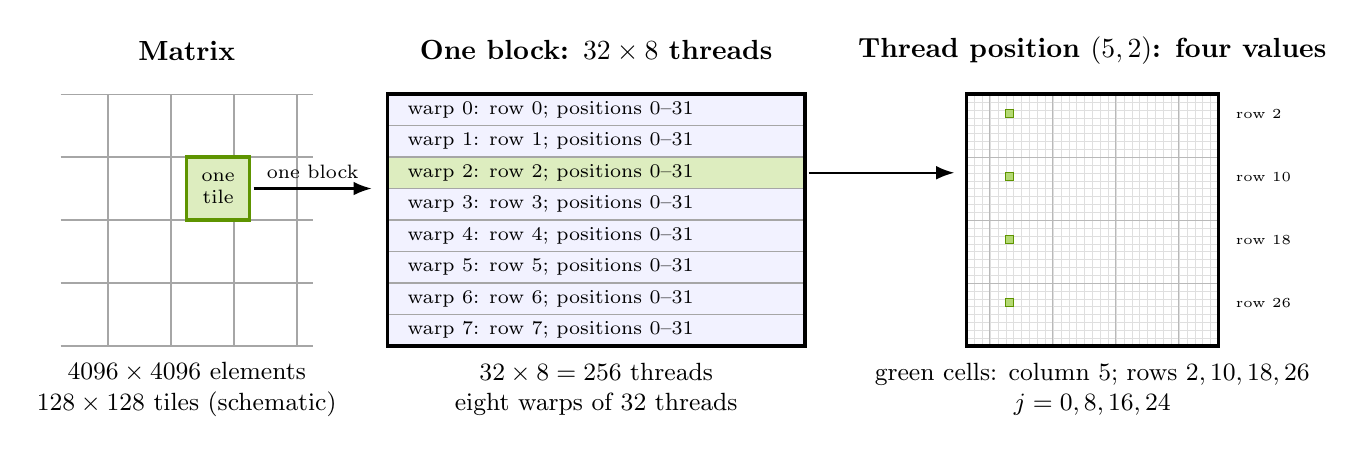
\begin{tikzpicture}[>=Latex,font=\small]
    % Matrix divided into tiles.
    \node[font=\bfseries] at (1.8,3.75) {Matrix};
    \draw[step=0.8,gray!70] (0.2,0) grid (3.4,3.2);
    \filldraw[fill=nvidiagreen!25,draw=nvidiagreen!80!black,very thick]
      (1.8,1.6) rectangle (2.6,2.4);
    \node[font=\scriptsize,align=center] at (2.2,2.0) {one\\tile};
    \node[align=center] at (1.8,-0.55)
      {$4096\times4096$ elements\\$128\times128$ tiles (schematic)};

    % One CUDA block, divided by the hardware into eight warps.
    \draw[->,thick] (2.65,2.0) -- (4.15,2.0)
      node[midway,above,font=\scriptsize] {one block};
    \node[font=\bfseries] at (7.0,3.75) {One block: $32\times8$ threads};
    \foreach \w in {0,...,7} {
      \pgfmathsetmacro{\ytop}{3.2-0.4*\w}
      \pgfmathsetmacro{\ybottom}{2.8-0.4*\w}
      \pgfmathsetmacro{\ymid}{3.0-0.4*\w}
      \ifnum\w=2
        \fill[nvidiagreen!25] (4.35,\ybottom) rectangle (9.65,\ytop);
      \else
        \fill[blue!5] (4.35,\ybottom) rectangle (9.65,\ytop);
      \fi
      \draw[gray!70] (4.35,\ybottom) rectangle (9.65,\ytop);
      \node[anchor=west,font=\scriptsize] at (4.48,\ymid)
        {warp \w: row \w; positions 0--31};
    }
    \draw[very thick] (4.35,0) rectangle (9.65,3.2);
    \node[align=center] at (7.0,-0.55)
      {$32\times8=256$ threads\\eight warps of 32 threads};

    % Four cells handled by one representative thread, shown on the tile.
    \draw[->,thick] (9.7,2.2) -- (11.55,2.2);
    \node[font=\bfseries] at (13.3,3.75) {Thread position $(5,2)$: four values};
    \draw[step=0.1,gray!25,line width=0.1pt] (11.7,0) grid (14.9,3.2);
    \draw[step=0.8,gray!55,line width=0.35pt] (11.7,0) grid (14.9,3.2);
    \draw[very thick] (11.7,0) rectangle (14.9,3.2);
    \foreach \rowindex in {2,10,18,26} {
      \pgfmathsetmacro{\celltop}{3.2-0.1*\rowindex}
      \pgfmathsetmacro{\cellbottom}{3.1-0.1*\rowindex}
      \pgfmathsetmacro{\cellmid}{3.15-0.1*\rowindex}
      \filldraw[fill=nvidiagreen!55,draw=nvidiagreen!80!black,line width=0.4pt]
        (12.2,\cellbottom) rectangle (12.3,\celltop);
      \node[anchor=west,font=\tiny] at (15.0,\cellmid) {row \rowindex};
    }
    \node[align=center] at (13.3,-0.55)
      {green cells: column 5; rows $2,10,18,26$\\$j=0,8,16,24$};
  \end{tikzpicture}%
  }
  \caption{One block covers the selected $32\times32$ tile.  Its 256 threads form
  eight warps.  Thread position $(5,2)$ means
  $(\code{threadIdx.x},\code{threadIdx.y})=(5,2)$.  That thread processes four rows
  because the block has 8 thread rows while the tile has 32 matrix rows.}
  \label{fig:transpose-tile-map}
\end{figure}
\FloatBarrier

The matrices are stored as flat row-major arrays, so matrix element
$(\text{row},\text{column})$ has index \code{row * n + column}.  The constants
\code{tile\_width = 32} and \code{block\_rows = 8} fix the tile and block shape.
The keyword \code{constexpr} marks both values as compile-time constants.  The
unoptimized kernel is
\begin{lstlisting}[language=CUDA,caption={One $32\times32$ matrix tile per $32\times8$-thread block.}]
constexpr int tile_width = 32;
constexpr int block_rows = 8;

__global__ void transpose_strided_write(const float* input,
                                        float* output, int n) {
  const int x = blockIdx.x * tile_width + threadIdx.x;
  const int y = blockIdx.y * tile_width + threadIdx.y;
  for (int j = 0; j < tile_width; j += block_rows) {
    // In a flat n-column matrix, (row, column) is row * n + column.
    // Copy input(row=y+j, column=x) to output(row=x, column=y+j).
    output[x * n + y + j] = input[(y + j) * n + x];
  }
}

constexpr int n = 4096;
const dim3 threads(tile_width, block_rows);       // (32, 8)
const dim3 blocks(n / tile_width, n / tile_width); // (128, 128)
transpose_strided_write<<<blocks, threads>>>(input, output, n);
\end{lstlisting}

The launch creates $128\times128$ blocks.  One block covers one $32\times32$ tile
with $32\times8=256$ threads.  Each row of 32 threads is one warp.  The loop values
$j=0,8,16,24$ make each thread process four rows, so the 256 threads cover all
$32\times32=1024$ values in the tile.

\Needspace{9\baselineskip}
To inspect one warp, hold \code{threadIdx.y} and $j$ fixed while
\code{threadIdx.x} runs from 0 to 31.  The variable $x$ then increases by one from
one thread to the next.  Therefore
\begin{itemize}
  \item the read index \code{(y + j) * n + x} increases by one, so the warp reads
  32 adjacent floats;
  \item the write index \code{x * n + y + j} increases by $n=4096$, so consecutive
  threads write 4096 floats, or $16\ \mathrm{KiB}$, apart.
\end{itemize}
The GPU serves the 32 adjacent reads with few memory requests.  This pattern is
called \emph{coalesced access}.  The writes are not adjacent.  One warp writes 32
floats to rows separated by 16~KiB, so the GPU needs many write requests
\cite{cuda-programming-guide,cuda-best-practices}.

The optimized kernel first reads adjacent values into shared memory.  It then reads
the shared array in the transposed direction and writes adjacent values to global
memory.  Shared memory changes the access direction between the coalesced global
read and the coalesced global write.

The extra shared-memory column is padding.  Without it, the transposed read asks
one part of shared memory for several different values at once, so those values are
returned one after another.  This is called a \emph{shared-memory bank conflict}.
Padding shifts the addresses so the values can be returned together
\cite{cuda-best-practices}.
\begin{lstlisting}[language=CUDA,basicstyle=\ttfamily\footnotesize,
  caption={Tiled transpose used in the experiment.}]
__global__ void transpose_tiled(const float* input, float* output, int n) {
  // Use 33 columns so column reads use different shared-memory banks.
  __shared__ float local[tile_width][tile_width + 1];
  int x = blockIdx.x * tile_width + threadIdx.x;
  int y = blockIdx.y * tile_width + threadIdx.y;
  for (int j = 0; j < tile_width; j += block_rows) {
    // Adjacent threads read adjacent input columns into shared memory.
    local[threadIdx.y + j][threadIdx.x] = input[(y + j) * n + x];
  }
  // Do not read the shared tile until every thread has finished writing it.
  __syncthreads();
  // Swap the block coordinates before writing the transposed square.
  x = blockIdx.y * tile_width + threadIdx.x;
  y = blockIdx.x * tile_width + threadIdx.y;
  for (int j = 0; j < tile_width; j += block_rows) {
    // Read rows as columns; adjacent threads now write adjacent output values.
    output[(y + j) * n + x] = local[threadIdx.x][threadIdx.y + j];
  }
}
\end{lstlisting}

In the first loop, the 32 threads read adjacent input values into shared memory.
After all threads finish that write, the second loop reads the shared array in the
other direction.  Its output index, \code{(y + j) * n + x}, increases by one from
thread to thread.  Both global-memory operations now use adjacent addresses.

\textbf{Measured result.}  On the office RTX 3090, the median of five process runs
gave $0.495\ \mathrm{ms}$ and $271.295\ \mathrm{GB/s}$ for the strided-write kernel,
versus $0.165\ \mathrm{ms}$ and $813.354\ \mathrm{GB/s}$ for the tiled kernel.  Each
process run reported the mean of 20 timed launches after one warm-up launch.  The
tiled kernel was $3.00\times$ faster because it replaced the far-apart global writes
with adjacent writes.  The raw output is in
\path{measurements/office_rtx3090_2026-09-01.txt} in the code repository.

\textbf{What to change.}  Make consecutive threads access consecutive values in
global memory.  For a transpose, use shared memory to change the direction between
the adjacent read and the adjacent write.

\FloatBarrier
% ----------------------------------------------------------------------------
\subsection{Warp divergence}
% ----------------------------------------------------------------------------

A warp executes one instruction for its 32 threads together.  If some threads
choose \code{branch\_a} and others choose \code{branch\_b}, the warp runs one
branch and then the other.  Only the threads that chose the current branch do work.
If all 32 threads choose the same branch, the other branch is skipped.  Running
both branches because one warp contains both choices is called \emph{warp divergence}
\cite{cuda-programming-guide}.

Both versions send half the threads to each function, and \code{branch\_a} and
\code{branch\_b} perform equal amounts of arithmetic.  Only the assignment of
threads to functions changes.  In the unoptimized kernel, neighboring thread
indices alternate between the two functions.
\begin{lstlisting}[language=CUDA,numbers=none,caption={Unoptimized.  One warp contains both branches.}]
// Adjacent thread indices alternate even, odd, even, odd, ...
const bool take_a = (index & 1) == 0;
output[index] = take_a ? branch_a(input[index])
                       : branch_b(input[index]);
\end{lstlisting}
The optimized kernel assigns one branch to a whole warp.
\begin{lstlisting}[language=CUDA,numbers=none,caption={Optimized.  All 32 threads in one warp agree.}]
// index / warpSize is identical for all 32 threads in one warp.
const bool take_a = ((index / warpSize) & 1) == 0;
output[index] = take_a ? branch_a(input[index])
                       : branch_b(input[index]);
\end{lstlisting}

Figure~\ref{fig:warp-divergence} shows how the two assignments change the work done
by each warp without changing the number of calls to either function.

\begin{figure}[htbp]
  \centering
  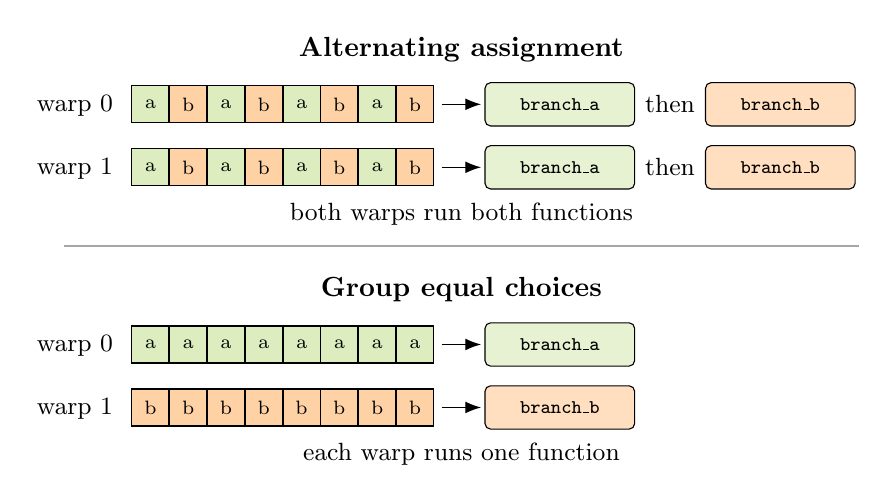
\begin{tikzpicture}[
    font=\small,
    thread/.style={draw,minimum width=4.7mm,minimum height=4.7mm,
      inner sep=0pt,font=\scriptsize},
    function/.style={draw,rounded corners=2pt,minimum width=19mm,
      minimum height=5.5mm,font=\ttfamily\scriptsize},
  ]
    \node[font=\bfseries] at (6.3,3.15) {Alternating assignment};
    \node[anchor=e] at (2.0,2.45) {warp 0};
    \node[anchor=e] at (2.0,1.65) {warp 1};
    \foreach \y in {2.45,1.65} {
      \foreach \i in {0,...,7} {
        \ifodd\i
          \node[thread,fill=orange!35] at (2.35+0.48*\i,\y) {b};
        \else
          \node[thread,fill=nvidiagreen!25] at (2.35+0.48*\i,\y) {a};
        \fi
      }
      \draw[-{Latex[length=2mm]}] (6.05,\y) -- (6.55,\y);
      \node[function,fill=nvidiagreen!18] at (7.55,\y) {branch\_a};
      \node at (8.95,\y) {then};
      \node[function,fill=orange!25] at (10.35,\y) {branch\_b};
    }
    \node[font=\small] at (6.3,1.05) {both warps run both functions};

    \draw[black!35] (1.25,0.65) -- (11.35,0.65);

    \node[font=\bfseries] at (6.3,0.10) {Group equal choices};
    \node[anchor=e] at (2.0,-0.60) {warp 0};
    \node[anchor=e] at (2.0,-1.40) {warp 1};
    \foreach \i in {0,...,7} {
      \node[thread,fill=nvidiagreen!25] at (2.35+0.48*\i,-0.60) {a};
      \node[thread,fill=orange!35] at (2.35+0.48*\i,-1.40) {b};
    }
    \draw[-{Latex[length=2mm]}] (6.05,-0.60) -- (6.55,-0.60);
    \draw[-{Latex[length=2mm]}] (6.05,-1.40) -- (6.55,-1.40);
    \node[function,fill=nvidiagreen!18] at (7.55,-0.60) {branch\_a};
    \node[function,fill=orange!25] at (7.55,-1.40) {branch\_b};
    \node[font=\small] at (6.3,-2.00) {each warp runs one function};
  \end{tikzpicture}
  \caption{With alternating choices, each warp runs \texttt{branch\_a} and then
  \texttt{branch\_b}.  After equal choices are grouped, warp 0 runs only
  \texttt{branch\_a} and warp 1 runs only \texttt{branch\_b}.  Each row shows eight
  of the warp's 32 threads.}
  \label{fig:warp-divergence}
\end{figure}
\FloatBarrier

\textbf{What to change.}
When possible, group the work so all threads in one warp choose the same branch.
Do not replace the branch with arithmetic unless the arithmetic replacement does
less work.

% ----------------------------------------------------------------------------
\subsection{Atomic contention}
% ----------------------------------------------------------------------------

Suppose two threads add 1 to the same counter.  If both read the old value $c$
before either writes, both compute $c+1$ and both write $c+1$.  The final value is
$c+1$ instead of $c+2$: one increment is lost.

\code{atomicAdd(counter, 1)} prevents the lost increment by completing one update
before another update to the same counter begins.  The answer is correct, but many
threads may wait for access to the counter.  This wait is called \emph{atomic
contention}~\cite{cuda-programming-guide}.

In the following snippets, \code{index} is the thread's global index and
\code{count} is the number of events.  The unoptimized kernel makes every valid
thread add 1 directly to the same counter in GPU memory.
\Needspace{11\baselineskip}
\begin{lstlisting}[language=CUDA,numbers=none,caption={Every valid thread updates the same counter.}]
if (index < count) {
  // Wait for a turn, then add 1 to the counter in GPU memory.
  atomicAdd(counter, 1ULL);
}
\end{lstlisting}
The program uses 256 threads per block.  Each thread first stores either 1 or 0 in
the block's shared memory.  The block adds those 256 values together.  Thread 0
then adds the block's total to \code{counter}.  A block therefore calls
\code{atomicAdd} once instead of as many as 256 times.
\begin{lstlisting}[language=CUDA,numbers=none,caption={Add inside the block, then update the counter once.}]
// Reserve one shared-memory entry for each thread.
__shared__ unsigned int local[256];
const int index = blockIdx.x * blockDim.x + threadIdx.x;
// Store 1 for a valid event and 0 otherwise.
local[threadIdx.x] = index < count ? 1U : 0U;
__syncthreads();
// Add pairs of entries until local[0] holds the block total.
for (int offset = blockDim.x / 2; offset > 0; offset /= 2) {
  if (threadIdx.x < offset) {
    local[threadIdx.x] += local[threadIdx.x + offset];
  }
  __syncthreads();
}
if (threadIdx.x == 0) {
  // Thread 0 adds the block total to the global counter once.
  atomicAdd(counter, (unsigned long long)local[0]);
}
\end{lstlisting}

Figure~\ref{fig:atomic-contention} compares the two versions.

\begin{figure}[htbp]
  \centering
  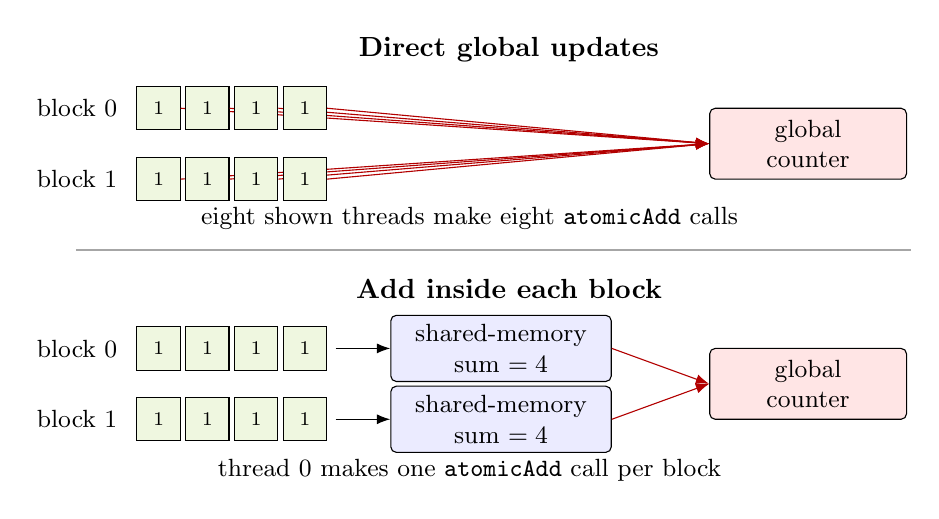
\begin{tikzpicture}[>=Latex,font=\small,
    thread/.style={draw,fill=nvidiagreen!12,minimum size=5.5mm,
      inner sep=0pt,font=\scriptsize},
    partial/.style={draw,rounded corners=2pt,fill=blue!8,
      minimum width=28mm,minimum height=7mm,align=center},
    counter/.style={draw,rounded corners=2pt,fill=red!10,
      minimum width=25mm,minimum height=9mm,align=center}]

    \node[font=\bfseries] at (6.2,3.20)
      {Direct global updates};
    \node[anchor=east] at (1.35,2.45) {block 0};
    \node[anchor=east] at (1.35,1.55) {block 1};
    \node[counter] (directcounter) at (10.0,2.00) {global\\counter};
    \foreach \row/\y in {0/2.45,1/1.55} {
      \foreach \i in {0,...,3} {
        \node[thread] (direct\row\i) at (1.75+0.62*\i,\y) {1};
        \draw[->,red!70!black] (direct\row\i.east) -- (directcounter.west);
      }
    }
    \node at (5.7,1.05)
      {eight shown threads make eight \code{atomicAdd} calls};

    \draw[black!35] (0.7,0.65) -- (11.3,0.65);

    \node[font=\bfseries] at (6.2,0.15)
      {Add inside each block};
    \node[anchor=east] at (1.35,-0.60) {block 0};
    \node[anchor=east] at (1.35,-1.50) {block 1};
    \foreach \row/\y in {0/-0.60,1/-1.50} {
      \foreach \i in {0,...,3}
        \node[thread] at (1.75+0.62*\i,\y) {1};
    }
    \node[partial] (sum0) at (6.10,-0.60) {shared-memory\\sum $=4$};
    \node[partial] (sum1) at (6.10,-1.50) {shared-memory\\sum $=4$};
    \draw[->] (4.00,-0.60) -- (sum0.west);
    \draw[->] (4.00,-1.50) -- (sum1.west);
    \node[counter] (reducedcounter) at (10.0,-1.05) {global\\counter};
    \draw[->,red!70!black] (sum0.east) -- (reducedcounter.west);
    \draw[->,red!70!black] (sum1.east) -- (reducedcounter.west);
    \node at (5.7,-2.15)
      {thread 0 makes one \code{atomicAdd} call per block};
  \end{tikzpicture}
  \caption{Four valid threads are shown for each block.  The direct-update version makes
  eight \texttt{atomicAdd} calls.  The block-sum version adds inside each block and makes only
  two calls.  The supplied code uses 256 threads per block.}
  \label{fig:atomic-contention}
\end{figure}
\FloatBarrier

\textbf{What to change.}
Add values together inside each block, then update the counter once per block.  If
every thread truly must update the same counter separately, changing the number of
blocks or threads cannot remove the wait.

% ----------------------------------------------------------------------------
\Needspace{10\baselineskip}
\subsection{Memory latency}
% ----------------------------------------------------------------------------

The example uses a chain of memory reads:
\begin{lstlisting}[language=CUDA,numbers=none,caption={Each read supplies the index for the next read.}]
int position = starting_position;
for (int step = 0; step < steps; ++step) {
  // next[position] must return before the next loop iteration can begin.
  position = next[position];
}
\end{lstlisting}
The value returned by \code{next[position]} becomes the index used by the next
iteration.  The thread cannot begin that next read early.  It must wait for the
current read to return.  The time between starting a read and receiving its value
is called \emph{memory latency}.

While one warp waits, the SM can run another warp.  The SM becomes idle only if all
warps currently on it are waiting.  The two programs perform the same reads with
the same total number of threads; only the block size changes.
\begin{center}
\begin{tabular}{@{}lcc@{}}
  \toprule
  & Threads per block & Warps supplied by each block \\
  \midrule
  Unoptimized & 32 & 1 \\
  Optimized & 256 & 8 \\
  \bottomrule
\end{tabular}
\end{center}
An SM can hold only a limited number of blocks at once.  With 32-thread blocks, it
can reach that block limit while holding relatively few warps.  The 256-thread
blocks provide more warps that can run while another warp waits
\cite{kirkhwu2010,ampere-tuning-guide}.  Figure~\ref{fig:latency-hiding} shows the
idea; it does not show the exact number of warps on an SM.

\begin{figure}[htbp]
  \centering
  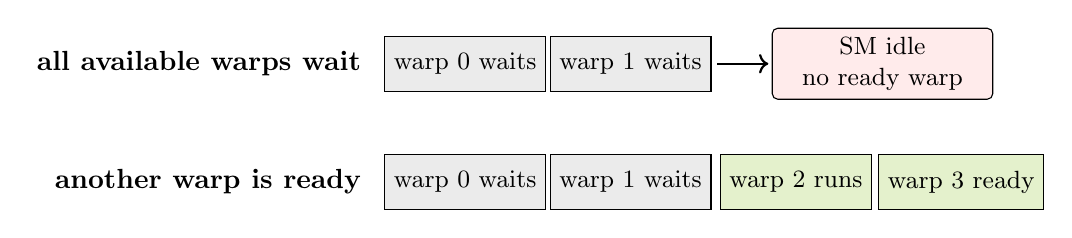
\begin{tikzpicture}[font=\small,
    run/.style={draw,fill=nvidiagreen!20,minimum width=19mm,minimum height=7mm},
    wait/.style={draw,fill=black!8,minimum width=19mm,minimum height=7mm},
    state/.style={draw,rounded corners=2pt,minimum width=28mm,minimum height=9mm,
      align=center}]
    \node[font=\bfseries,anchor=east] at (-0.2,1.15) {all available warps wait};
    \node[wait] at (1.0,1.15) {warp 0 waits};
    \node[wait] at (3.1,1.15) {warp 1 waits};
    \node[state,fill=red!8] at (6.3,1.15) {SM idle\\no ready warp};
    \draw[->,thick] (4.2,1.15)--(4.85,1.15);

    \node[font=\bfseries,anchor=east] at (-0.2,-0.35) {another warp is ready};
    \node[wait] at (1.0,-0.35) {warp 0 waits};
    \node[wait] at (3.1,-0.35) {warp 1 waits};
    \node[run] at (5.2,-0.35) {warp 2 runs};
    \node[run] at (7.3,-0.35) {warp 3 ready};
  \end{tikzpicture}
  \caption{If every available warp is waiting, the SM is idle.  Another ready warp
  gives the SM work to run during the wait.  The figure is schematic.}
  \label{fig:latency-hiding}
\end{figure}
\FloatBarrier

\textbf{What to change.}
Choose a block size that lets each SM hold enough warps to provide other work during
a memory wait.  Nsight Compute calls the fraction of the SM's thread capacity in
use \emph{occupancy}.  Maximum occupancy is not the goal: once a ready warp is
usually available, adding more warps may not make the kernel faster.

% ----------------------------------------------------------------------------
\subsection{Kernel launch overhead}
% ----------------------------------------------------------------------------

The CPU and CUDA driver need time to submit each kernel.  The CPU does not wait for
the submitted kernel to finish.  The time needed to submit one kernel is called
\emph{launch overhead}.  If each kernel finishes before the CPU can submit the next
kernel, the GPU sits idle between kernels.  Adding blocks to the tiny kernels does
not remove the gaps between launches.

The supplied example uses 10,000 steps to make the launch cost easy to see.  The
step count is an example parameter, not a measured hardware limit.  The unoptimized
CPU loop submits one kernel per step.
\begin{lstlisting}[language=CUDA,numbers=none,caption={Unoptimized.  Pay the launch cost on every step.}]
// The CPU submits a separate kernel launch for every tiny step.
for (int step = 0; step < 10000; ++step) {
  one_tiny_step<<<1, 32>>>(value);
}
\end{lstlisting}
The optimized version submits once and moves the loop into the kernel.
\begin{lstlisting}[language=CUDA,numbers=none,caption={Optimized.  One launch performs all 10,000 steps.}]
__global__ void fused_tiny_steps(float* value, int steps) {
  // One thread performs the same 10,000 updates inside one kernel launch.
  if (blockIdx.x == 0 && threadIdx.x == 0) {
    float result = value[0];
    for (int step = 0; step < steps; ++step) {
      result += 1.0f;
    }
    value[0] = result;
  }
}

// The CPU now pays the launch cost once.
fused_tiny_steps<<<1, 32>>>(value, 10000);
\end{lstlisting}

Figure~\ref{fig:launch-overhead} shows what the CPU and GPU do over time in the two
versions.

\begin{figure}[htbp]
  \centering
  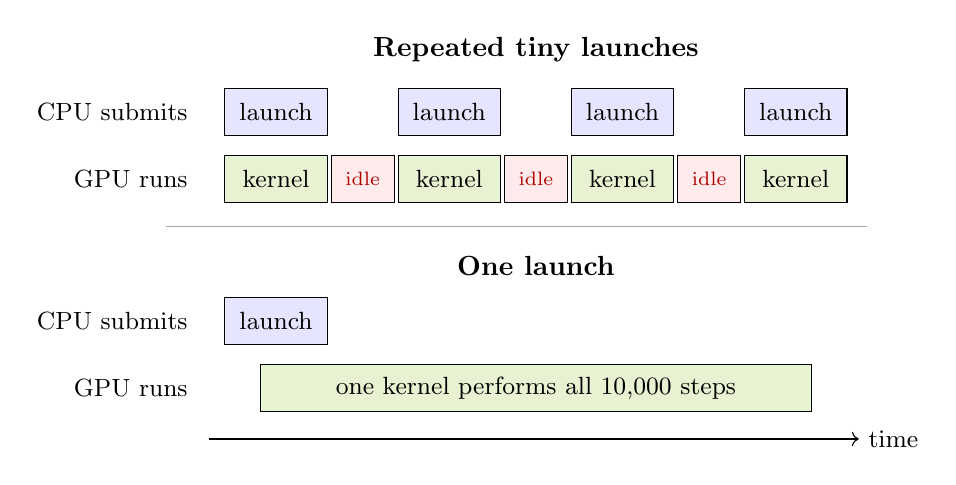
\begin{tikzpicture}[font=\small,
    host/.style={draw,fill=blue!10,minimum height=6mm,minimum width=13mm},
    gpu/.style={draw,fill=nvidiagreen!18,minimum height=6mm,minimum width=13mm},
    idle/.style={draw,fill=red!8,text=red!70!black,minimum height=6mm,
      minimum width=8mm,font=\scriptsize}]
    \node[font=\bfseries] at (4.3,2.00) {Repeated tiny launches};
    \node[anchor=east] at (0,1.20) {CPU submits};
    \node[anchor=east] at (0,0.35) {GPU runs};
    \foreach \x in {1.0,3.2,5.4,7.6}
      \node[host] at (\x,1.20) {launch};
    \foreach \x in {1.0,3.2,5.4,7.6}
      \node[gpu] at (\x,0.35) {kernel};
    \foreach \x in {2.1,4.3,6.5}
      \node[idle] at (\x,0.35) {idle};

    \draw[black!35] (-0.4,-0.25) -- (8.5,-0.25);

    \node[font=\bfseries] at (4.3,-0.75) {One launch};
    \node[anchor=east] at (0,-1.45) {CPU submits};
    \node[anchor=east] at (0,-2.30) {GPU runs};
    \node[host] at (1.0,-1.45) {launch};
    \node[gpu,minimum width=70mm] at (4.3,-2.30)
      {one kernel performs all 10,000 steps};
    \draw[->] (0.15,-2.95) -- (8.4,-2.95) node[right] {time};
  \end{tikzpicture}
  \caption{With repeated tiny launches, the GPU is idle in the red intervals while
  waiting for the CPU to submit more work.  The combined version pays for one
  launch and runs one longer kernel.}
  \label{fig:launch-overhead}
\end{figure}
\FloatBarrier

\textbf{What to change.}
Put several small steps in one kernel when possible.  A CUDA Graph records a
repeated group of launches and lets the CPU submit the group with less repeated
work.  Nsight Systems shows the CPU launch calls and the idle gaps on the GPU timeline
\cite{cuda-graphs2021}.

% ----------------------------------------------------------------------------
\subsection{Host-device transfer overhead}
% ----------------------------------------------------------------------------

Copying an array between CPU and GPU memory can take longer than running a kernel on
the array.  A program that copies both inputs to the GPU and the result back on every
step may therefore spend most of its time copying.  The input and output copies
usually cross Peripheral Component Interconnect Express (PCIe), not the GPU's own
device-memory connection.  The copy time is called \emph{host-device transfer
overhead}.  Measure the copies as well as the kernel.

The supplied programs choose 20 steps.  The unoptimized CPU loop makes three copies
per step across PCIe.
\begin{lstlisting}[language=CUDA,numbers=none,caption={Unoptimized.  Transfer on every iteration.}]
for (int step = 0; step < 20; ++step) {
  // Move both inputs to the GPU again on every iteration.
  cudaMemcpy(x, host_x, bytes, cudaMemcpyHostToDevice);
  cudaMemcpy(y, host_y, bytes, cudaMemcpyHostToDevice);
  vector_add<<<blocks, threads>>>(x, y, output, count);
  // Move the result back before starting the next iteration.
  cudaMemcpy(host_output, output, bytes, cudaMemcpyDeviceToHost);
}
\end{lstlisting}
The optimized host code leaves the arrays on the GPU between kernel launches.
\begin{lstlisting}[language=CUDA,numbers=none,caption={Optimized.  Transfer inputs and output only once.}]
// Copy the inputs once and leave them in GPU memory.
cudaMemcpy(x, host_x, bytes, cudaMemcpyHostToDevice);
cudaMemcpy(y, host_y, bytes, cudaMemcpyHostToDevice);
for (int step = 0; step < 20; ++step) {
  vector_add<<<blocks, threads>>>(x, y, output, count);
}
// Copy the final result back after all 20 launches.
cudaMemcpy(host_output, output, bytes, cudaMemcpyDeviceToHost);
\end{lstlisting}

Figure~\ref{fig:transfer-bound} shows which transfers disappear when the arrays
remain on the GPU between launches.

\begin{figure}[htbp]
  \centering
  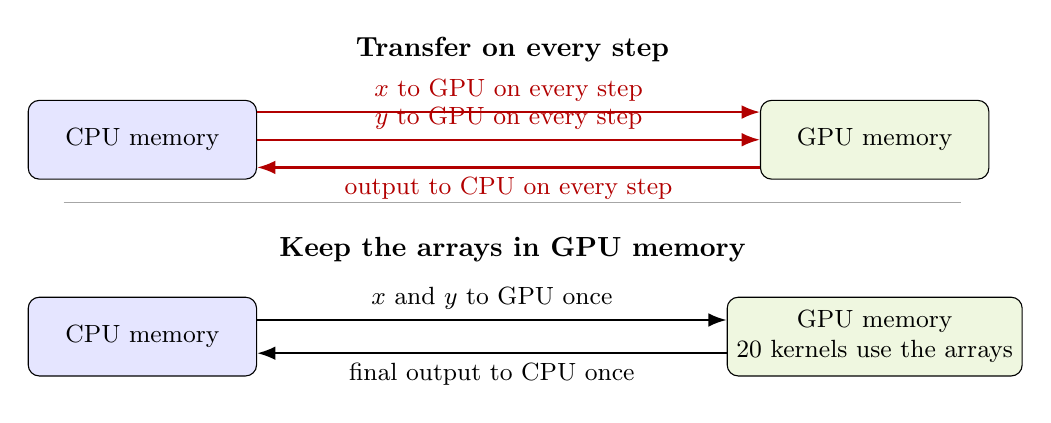
\begin{tikzpicture}[>=Latex,font=\small,
    memory/.style={draw,rounded corners,minimum width=29mm,minimum height=10mm,
      align=center}]
    \node[font=\bfseries] at (6.3,2.00) {Transfer on every step};
    \node[memory,fill=blue!10] (h1) at (1.6,0.85) {CPU memory};
    \node[memory,fill=nvidiagreen!12] (d1) at (10.9,0.85) {GPU memory};
    \draw[->,red!70!black,thick] ([yshift=10pt]h1.east) --
      node[above]{$x$ to GPU on every step} ([yshift=10pt]d1.west);
    \draw[->,red!70!black,thick] (h1.east) --
      node[above]{$y$ to GPU on every step} (d1.west);
    \draw[<-,red!70!black,thick] ([yshift=-10pt]h1.east) --
      node[below]{output to CPU on every step} ([yshift=-10pt]d1.west);

    \draw[black!35] (0.6,0.05) -- (12.0,0.05);

    \node[font=\bfseries] at (6.3,-0.55) {Keep the arrays in GPU memory};
    \node[memory,fill=blue!10] (h2) at (1.6,-1.65) {CPU memory};
    \node[memory,fill=nvidiagreen!12] (d2) at (10.9,-1.65)
      {GPU memory\\20 kernels use the arrays};
    \draw[->,thick] ([yshift=6pt]h2.east) --
      node[above]{$x$ and $y$ to GPU once} ([yshift=6pt]d2.west);
    \draw[<-,thick] ([yshift=-6pt]h2.east) --
      node[below]{final output to CPU once} ([yshift=-6pt]d2.west);
  \end{tikzpicture}
  \caption{Keeping the arrays in GPU memory removes the repeated transfers between
  consecutive kernel launches.}
  \label{fig:transfer-bound}
\end{figure}
\FloatBarrier

Both programs use the same kind of CPU memory.  The only difference being tested is
how often the arrays are copied.

\textbf{What to change.}
Leave arrays in GPU memory while consecutive kernels use them.  Copy back only the
values the CPU actually needs~\cite{cuda-best-practices}.

% ============================================================================
\section*{Sources}
\addcontentsline{toc}{section}{Sources}
% ============================================================================

The CUDA Refresher posts supply the CPU and GPU model, library map, and programming
model.  NVIDIA's updated CUDA introduction supplies the array-addition example.
Betcke and Scroggs explain the connection between warps and SMs.  NVIDIA's Ampere
article supplies the GA100 and A100 architecture.  NVIDIA's GA102 whitepaper and
RTX 3090 specifications supply the consumer-GPU comparison.

He supplies the three names compute-bound, memory-bound, and overhead-bound.
Current NVIDIA documentation supplies the tool names and CUDA behavior used in
Section~\ref{sec:gpu-underutilization}.  Kirk and Hwu's textbook explains why an SM
can run another warp while one warp waits for memory.

Williams, Waterman, and Patterson supply the roofline model.  The saved RTX 3090
measurement record supplies the four points in Figure~\ref{fig:measured-roofline}.

\textbf{Further reading.}
NVIDIA's \href{https://docs.nvidia.com/cuda/cuda-c-programming-guide/}%
{CUDA C++ Programming Guide} and
\href{https://docs.nvidia.com/cuda/cuda-c-best-practices-guide/}%
{CUDA C++ Best Practices Guide} are the natural next references.

\begingroup
\small
\raggedright
\begin{thebibliography}{99}

\bibitem{gupta2020origins}
Pradeep Gupta.
\newblock \emph{CUDA Refresher: Reviewing the Origins of GPU Computing}.
\newblock NVIDIA Technical Blog, April 23, 2020.
\newblock \url{https://developer.nvidia.com/blog/cuda-refresher-reviewing-the-origins-of-gpu-computing/}.

\bibitem{gupta2020gettingstarted}
Pradeep Gupta.
\newblock \emph{CUDA Refresher: Getting Started with CUDA}.
\newblock NVIDIA Technical Blog, May 6, 2020.
\newblock \url{https://developer.nvidia.com/blog/cuda-refresher-getting-started-with-cuda/}.

\bibitem{gupta2020ecosystem}
Pradeep Gupta.
\newblock \emph{CUDA Refresher: The GPU Computing Ecosystem}.
\newblock NVIDIA Technical Blog, May 21, 2020.
\newblock \url{https://developer.nvidia.com/blog/cuda-refresher-the-gpu-computing-ecosystem/}.

\bibitem{gupta2020model}
Pradeep Gupta.
\newblock \emph{CUDA Refresher: The CUDA Programming Model}.
\newblock NVIDIA Technical Blog, June 26, 2020.
\newblock \url{https://developer.nvidia.com/blog/cuda-refresher-the-cuda-programming-model/}.

\bibitem{harris2025cuda}
Mark Harris.
\newblock \emph{An Even Easier Introduction to CUDA (Updated)}.
\newblock NVIDIA Technical Blog, May 2, 2025.
\newblock \url{https://developer.nvidia.com/blog/even-easier-introduction-cuda/}.
\newblock Accessed August 24, 2026.

\bibitem{betcke2022cuda}
Timo Betcke and Matthew Scroggs.
\newblock \emph{A Tour of CUDA}.
\newblock Techniques of High-Performance Computing lecture notes, 2020--2022.
\newblock \url{https://tbetcke.github.io/hpc_lecture_notes/cuda_introduction.html}.
\newblock Accessed August 25, 2026.

\bibitem{ampere2020}
Ronny Krashinsky, Olivier Giroux, Stephen Jones, Nick Stam, and Sridhar Ramaswamy.
\newblock \emph{NVIDIA Ampere Architecture In-Depth}.
\newblock NVIDIA Technical Blog, May 14, 2020.
\newblock \url{https://developer.nvidia.com/blog/nvidia-ampere-architecture-in-depth/}.

\bibitem{ga102whitepaper}
NVIDIA Corporation.
\newblock \emph{NVIDIA Ampere GA102 GPU Architecture}.
\newblock Architecture whitepaper, version 2.1, 2021.
\newblock \url{https://www.nvidia.com/content/PDF/nvidia-ampere-ga-102-gpu-architecture-whitepaper-v2.1.pdf}.
\newblock Accessed August 26, 2026.

\bibitem{rtx3090specs}
NVIDIA Corporation.
\newblock \emph{GeForce RTX 3090 Family Specifications}.
\newblock \url{https://www.nvidia.com/en-us/geforce/graphics-cards/30-series/rtx-3090-3090ti/}.
\newblock Accessed August 26, 2026.

\bibitem{he2022brrrr}
Horace He.
\newblock \emph{Making Deep Learning Go Brrrr From First Principles}.
\newblock 2022.
\newblock \url{https://horace.io/brrr_intro.html}.
\newblock Accessed August 25, 2026.

\bibitem{williams2009roofline}
Samuel Williams, Andrew Waterman, and David Patterson.
\newblock \emph{Roofline: An Insightful Visual Performance Model for Multicore
Architectures}.
\newblock Communications of the ACM, 52(4):65--76, April 2009.
\newblock \url{https://doi.org/10.1145/1498765.1498785}.

\bibitem{roofline-measurement}
Measurement record.
\newblock \emph{Roofline Measurements on the Office RTX 3090}.
\newblock September 1, 2026.
\newblock Raw output and derivation in
\url{https://github.com/HaowuDuan/cuda-example-for-note},
\path{measurements/roofline_rtx3090_2026-09-01.txt}.

\bibitem{kirkhwu2010}
David B. Kirk and Wen-mei W. Hwu.
\newblock \emph{Programming Massively Parallel Processors: A Hands-on Approach}.
\newblock Morgan Kaufmann, 2010.
\newblock ISBN 978-0-12-381472-2.

\bibitem{cuda-programming-guide}
NVIDIA Corporation.
\newblock \emph{CUDA Programming Guide}.
\newblock \url{https://docs.nvidia.com/cuda/cuda-programming-guide/index.html}.
\newblock Accessed August 24, 2026.

\bibitem{cuda-gpus}
NVIDIA Corporation.
\newblock \emph{CUDA GPU Compute Capability}.
\newblock \url{https://developer.nvidia.com/cuda/gpus}.
\newblock Accessed September 1, 2026.

\bibitem{ampere-tuning-guide}
NVIDIA Corporation.
\newblock \emph{NVIDIA Ampere GPU Architecture Tuning Guide}.
\newblock \url{https://docs.nvidia.com/cuda/ampere-tuning-guide/index.html}.
\newblock Accessed September 1, 2026.

\bibitem{cuda-memory-model}
NVIDIA Corporation.
\newblock \emph{CUDA C++ Memory Model}.
\newblock \url{https://docs.nvidia.com/cuda/cuda-programming-guide/05-appendices/cuda-cpp-memory-model.html}.
\newblock Accessed August 24, 2026.

\bibitem{cuda-best-practices}
NVIDIA Corporation.
\newblock \emph{CUDA C++ Best Practices Guide}.
\newblock \url{https://docs.nvidia.com/cuda/cuda-c-best-practices-guide/index.html}.
\newblock Accessed August 26, 2026.

\bibitem{nsightcompute-profiling}
NVIDIA Corporation.
\newblock \emph{Nsight Compute Profiling Guide}.
\newblock \url{https://docs.nvidia.com/nsight-compute/ProfilingGuide/index.html}.
\newblock Accessed August 26, 2026.

\bibitem{cuda-graphs2021}
NVIDIA Corporation.
\newblock \emph{Employing CUDA Graphs in a Dynamic Environment}.
\newblock NVIDIA Technical Blog, October 21, 2021.
\newblock \url{https://developer.nvidia.com/blog/employing-cuda-graphs-in-a-dynamic-environment/}.
\newblock Accessed August 26, 2026.

\bibitem{cudax2026}
NVIDIA Corporation.
\newblock \emph{NVIDIA CUDA-X Libraries}.
\newblock \url{https://developer.nvidia.com/cuda/cuda-x-libraries}.
\newblock Accessed August 24, 2026.

\bibitem{nsightsystems2026}
NVIDIA Corporation.
\newblock \emph{NVIDIA Nsight Systems}.
\newblock \url{https://developer.nvidia.com/nsight-systems}.
\newblock Accessed August 24, 2026.

\bibitem{nsightcompute2026}
NVIDIA Corporation.
\newblock \emph{NVIDIA Nsight Compute}.
\newblock \url{https://developer.nvidia.com/nsight-compute/}.
\newblock Accessed August 24, 2026.

\bibitem{computesanitizer2026}
NVIDIA Corporation.
\newblock \emph{Compute Sanitizer}.
\newblock \url{https://docs.nvidia.com/compute-sanitizer/ComputeSanitizer/index.html}.
\newblock Accessed August 24, 2026.

\end{thebibliography}
\endgroup

\end{document}
